\documentclass{article}

% Language and encoding
\usepackage[spanish]{babel}
\usepackage[utf8]{inputenc}
\usepackage[T1]{fontenc}

% Set page size and margins
\usepackage[letterpaper,top=2cm,bottom=2cm,left=3cm,right=3cm,marginparwidth=1.75cm]{geometry}

% Useful packages
\PassOptionsToPackage{colorlinks=true,allcolors=blue}{hyperref}
\usepackage{amsmath}
\usepackage{amssymb}
\usepackage{graphicx}
\graphicspath{{Imagenes/}}
\usepackage{float}
\usepackage{attachfile}
\usepackage{pdfpages}
\usepackage[utf8]{inputenc}
\usepackage[T1]{fontenc}
\usepackage[spanish]{babel}
\usepackage{geometry}
\usepackage{graphicx}
\usepackage{booktabs}
\usepackage{longtable}
\usepackage{array}
\usepackage{xcolor}
\usepackage{colortbl}
\usepackage{fancyhdr}
\usepackage{titlesec}
\usepackage{hyperref}
\usepackage{listings}
% Permitir codificación UTF-8 dentro de los entornos listings
\lstset{inputencoding=utf8, extendedchars=true}
\usepackage{enumitem}
\usepackage{float}
\usepackage{caption}
\usepackage{subcaption}
\usepackage{multirow}
\usepackage{amsmath}

\usepackage{parskip}

% Hyperref should always go last
\usepackage{hyperref}

% Paragraph spacing
\setlength{\parskip}{0.8em}
\setlength{\parindent}{1.5em}

\title{Proyecto Final\\
Diseño e Implementación de Arquitectura NoSQL Geoespacial para Análisis de Potencial Solar en Territorios PDET}
\author{Daniel González, Eduardo De Brigard, Juan Pablo Hernández}

% ── Colores ───────────────────────────────────────────────────────────────────
\definecolor{azul}{RGB}{0,0,0}
\definecolor{azulclaro}{RGB}{0,0,0}
\definecolor{grisclaro}{RGB}{214,228,240}
\definecolor{grisfilas}{RGB}{242,247,251}
\definecolor{codebg}{RGB}{245,245,245}
\definecolor{codeframe}{RGB}{180,180,180}
\definecolor{verde}{RGB}{0,128,0}
\definecolor{rojo}{RGB}{192,0,0}

% ── Listings (código) ─────────────────────────────────────────────────────────
\lstset{
  backgroundcolor=\color{codebg},
  frame=single,
  rulecolor=\color{codeframe},
  basicstyle=\ttfamily\small,
  keywordstyle=\color{azulclaro}\bfseries,
  commentstyle=\color{verde}\itshape,
  stringstyle=\color{rojo},
  breaklines=true,
  showstringspaces=false,
  numbers=left,
  numberstyle=\tiny\color{gray},
  numbersep=5pt,
  tabsize=4,
  captionpos=b
}

\lstdefinelanguage{JavaScript}{
  keywords={const,let,var,function,return,if,else,for,while,new,true,false,null},
  morecomment=[l]{//},
  morestring=[b]"
}

% ── Hyperref ─────────────────────────────────────────────────────────────────
\hypersetup{
  colorlinks=true,
  linkcolor=azulclaro,
  urlcolor=azulclaro,
  citecolor=azulclaro
}

% ── Comando para celdas de encabezado de tabla ────────────────────────────────
\newcommand{\tblhdr}[1]{%
  \cellcolor{azulclaro}\textbf{\textcolor{white}{#1}}%
}
\newcommand{\tblhdraz}[1]{%
  \cellcolor{azul}\textbf{\textcolor{white}{#1}}%
}

% ══════════════════════════════════════════════════════════════════════════════








\begin{document}
\maketitle

\section{Introducción}

En el marco de la transición energética impulsada por la Unidad de Planeación Minero Energética (UPME), surge la necesidad de identificar zonas estratégicas para el despliegue de infraestructura de energía renovable en Colombia. Este proyecto se enfoca específicamente en evaluar el potencial de generación solar en los techos de edificaciones dentro de los territorios priorizados por los Programas de Desarrollo con Enfoque Territorial (PDET), buscando promover la equidad territorial y el desarrollo en regiones históricamente vulnerables.  El principal desafío técnico radica en el procesamiento masivo de datos. Para estimar el área disponible para paneles solares, es necesario integrar y comparar datasets globales que contienen miles de millones de registros de huellas de edificios (como Google Open Buildings y Microsoft Building Footprints), junto con la delimitación administrativa del DANE.  Dada la escala de la información y la naturaleza geográfica de los datos, este documento presenta una propuesta basada en tecnologías NoSQL, específicamente utilizando MongoDB. El uso de este paradigma permite una gestión flexible de esquemas y, sobre todo, una ejecución eficiente de operaciones espaciales complejas, fundamentales para cruzar los límites municipales con las estructuras detectadas por satélite.


\section{Diseño del esquema de base de datos NoSQL y plan de implementación}

 \subsection{Plan de Implementación}

\begin{enumerate}
    \item \textbf{Preparación de la Infraestructura NoSQL}
    \begin{itemize}
        \item Despliegue de MongoDB: Configuración de una instancia de base de datos orientada a documentos para el almacenamiento masivo de datos vectoriales.
        \item Indexación Espacial: Implementación de índices de tipo \texttt{2dsphere} para optimizar las consultas de proximidad y contención geográfica.
    \end{itemize}

    \item \textbf{Adquisición e Integración de Datos Territoriales}
    \begin{itemize}
        \item Filtro PDET: Procesamiento del Marco Geoestadístico Nacional (MGN) del DANE para extraer y limpiar los límites de los municipios priorizados como territorios PDET.
        \item Ingesta de Huellas de Edificios: Carga y normalización de al menos dos de los datasets globales (Microsoft Building Footprints y Google Open Buildings) en la base de datos NoSQL.
        \item Verificación de Integridad: Validación de formatos estructurales, topología de geometrías y consistencia de códigos DIVIPOLA para asegurar la integridad referencial y la precisión espacial de los datos territoriales integrados en el esquema NoSQL.
    \end{itemize}

    \item \textbf{Procesamiento y Análisis Geoespacial}
    \begin{itemize}
        \item Intersección Espacial: Ejecución de operaciones de filtrado para identificar exclusivamente las estructuras ubicadas dentro de los polígonos municipales PDET.
        \item Cálculo de Áreas: Estimación de la superficie de los techos y conteo total de edificaciones por cada jurisdicción seleccionada.
    \end{itemize}

    \item \textbf{Evaluación y Comparativa de Fuentes}
    \begin{itemize}
        \item Auditoría de Datos (EDA): Realización de un análisis exploratorio para comparar la precisión y el volumen de detecciones entre los datasets seleccionados.
        \item Análisis de Discrepancias: Definición de métricas de validación para identificar variaciones en la detección de estructuras y determinar la fuente con mayor confiabilidad para el cálculo de áreas solares en los municipios seleccionados.
    \end{itemize}

    \item \textbf{Consolidación de Resultados}
    \begin{itemize}
        \item Generación de Reportes: Creación de visualizaciones cartográficas y tablas de resumen que identifiquen los municipios con mayor potencial para granjas solares.
        \item Documentación de Recomendaciones: Redacción de hallazgos técnicos alineados con los objetivos de transición energética y equidad territorial de la UPME.
    \end{itemize}
\end{enumerate}

\subsection{Diseño del Modelo de Datos}

\subsubsection{A. Representación del Modelo (Estructura de Documentos)}

A continuación, se presentan las colecciones principales definidas para el almacenamiento y procesamiento de información geoespacial dentro del entorno NoSQL propuesto.

\textbf{Colección: territorios\_pdet}

\begin{itemize}
    \item \texttt{\_id}: Identificador único (ObjectId)
    \item \texttt{codigo\_mgn}: Código municipal del DANE
    \item \texttt{nombre\_municipio}: Nombre oficial
    \item \texttt{geometria\_pdet}: Objeto GeoJSON (MultiPolygon) que define los límites del municipio
    \item \texttt{datos\_pdet}: Información sobre el programa de desarrollo
\end{itemize}

\textbf{Colección: huellas\_edificios}
\begin{itemize}
    \item \texttt{\_id}: Identificador único (ObjectId)
    \item \texttt{fuente}: Origen del dato (Microsoft o Google)
    \item \texttt{geometria\_edificio}: Objeto GeoJSON (Polygon) con la huella del edificio
    \item \texttt{area\_estimada\_m2}: Valor numérico calculado para el potencial solar
    \item \texttt{metadata}: Confianza de detección y fecha de captura
\end{itemize}

\begin{figure}[h]
    \centering
    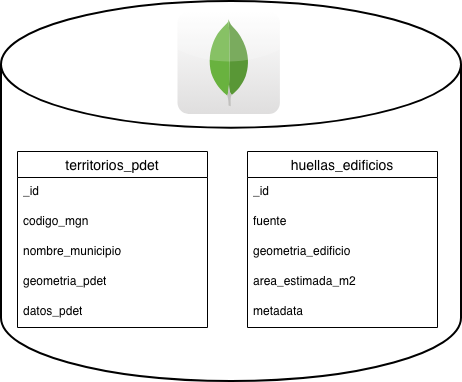
\includegraphics[width=0.6\textwidth]{Imagenes/colecciones.drawio.png}
    \caption{Esquema de base de datos}
\end{figure}

\subsubsection{B. Instrumento de Modelado: Relación Espacial}

En este modelo, la relación no se define mediante claves foráneas como en bases de datos relacionales, sino mediante una lógica de contención espacial:

\begin{itemize}
    \item \textbf{Vínculo lógico}: Un documento en \texttt{huellas\_edificios} pertenece a un territorio en \texttt{territorios\_pdet} si su \texttt{geometria\_edificio} está contenida dentro de \texttt{geometria\_pdet}.
    
    \item \textbf{Mecanismo de consulta}: Se utilizará el operador \texttt{\$geoWithin} de MongoDB para realizar el cruce de datos en tiempo de ejecución, evitando redundancia innecesaria.
\end{itemize}

\subsection{Esquema de Datos y Justificación}

Para cumplir con el requerimiento de una solución escalable y eficiente en operaciones espaciales, se ha diseñado un esquema basado en dos colecciones principales dentro de MongoDB.

\subsubsection{Descripción de las Colecciones}

\textbf{Colección: pdet\_territories}
\begin{itemize}
    \item \textbf{Propósito}: Almacenar los límites administrativos de los municipios designados como PDET, derivados del Marco Geoestadístico Nacional (MGN) del DANE.
    
    \item \textbf{Contenido}: Documentos que contienen el código municipal, nombre oficial y un campo \texttt{geometry} de tipo MultiPolygon bajo el estándar GeoJSON.
    
    \item \textbf{Índice}: Se implementará un índice \texttt{2dsphere} sobre el campo de geometría para permitir consultas de contención rápidas.
\end{itemize}

\textbf{Colección: building\_footprints}
\begin{itemize}
    \item \textbf{Propósito}: Consolidar las detecciones de edificios de los datasets de Google Open Buildings y Microsoft Building Footprints para su comparación.
    
    \item \textbf{Contenido}: Documentos con la huella del edificio (\texttt{Polygon}), el área calculada, la fuente del dato y metadatos de confianza.
    
    \item \textbf{Optimización}: Se incluirá un campo con el código municipal (obtenido tras el procesamiento inicial) para facilitar agregaciones estadísticas sin necesidad de realizar cruces espaciales en cada consulta.
\end{itemize}

\subsubsection{Justificación Técnica}

La elección de este esquema y del motor NoSQL (MongoDB) se fundamenta en los siguientes pilares:

\begin{itemize}

    \item \textbf{Soporte nativo geoespacial}: A diferencia de las bases de datos relacionales tradicionales, MongoDB maneja objetos GeoJSON de forma nativa. Esto facilita la ejecución de operadores como \texttt{\$geoWithin} y \texttt{\$geoIntersects}, esenciales para determinar qué edificios pertenecen a cada municipio PDET.

    \item \textbf{Escalabilidad}: El proyecto requiere procesar millones de registros provenientes de datasets globales de huellas de edificios. MongoDB permite manejar grandes volúmenes de información geoespacial de forma distribuida y eficiente.

    \item \textbf{Flexibilidad de esquema}: Debido a que los datasets utilizados provienen de múltiples fuentes (Google y Microsoft), existen diferencias estructurales y variaciones en atributos. El modelo orientado a documentos facilita la integración de estructuras heterogéneas sin requerir migraciones complejas.

    \item \textbf{Optimización de consultas espaciales}: La implementación de índices \texttt{2dsphere} permite acelerar operaciones de proximidad, intersección y contención espacial sobre polígonos territoriales y huellas de edificaciones.

    \item \textbf{Compatibilidad con pipelines geoespaciales}: El uso de GeoJSON facilita la interoperabilidad entre herramientas como QGIS, GeoPandas y MongoDB, permitiendo mantener consistencia espacial durante todas las etapas del procesamiento.

\end{itemize}
 
\subsection{Integración de Datos Territoriales y Filtro PDET}

En continuidad con el plan de implementación, se llevó a cabo la integración de la información geoespacial base para disponer de una colección preparada para análisis e ingesta en el entorno NoSQL.

\subsubsection{Metodología de procesamiento y normalización}
Para seleccionar los territorios priorizados se automatizó el cruce entre el Marco Geoestadístico Nacional (MGN) 2025 del DANE y el listado oficial de municipios PDET mediante scripts reproducibles en Python utilizando GeoPandas, Pandas y Matplotlib.

El flujo implementado permitió garantizar consistencia territorial, normalización de atributos y preparación geoespacial para posteriores procesos de ingesta en MongoDB.

Las acciones principales realizadas durante el procesamiento fueron:

\begin{itemize}
    \item Estandarización de códigos DIVIPOLA.
    \item Limpieza de nombres territoriales.
    \item Eliminación de caracteres Unicode y tildes.
    \item Validación de coincidencias territoriales.
    \item Conversión geoespacial a formato GeoJSON.
\end{itemize}

\vspace{0.3cm}

Como insumo principal del proceso se utilizó la capa administrativa nacional correspondiente al archivo:

\begin{center}
\texttt{MGN\_ADM\_MPIO\_GRAFICO.shp}
\end{center}

\begin{figure}[H]
    \centering
    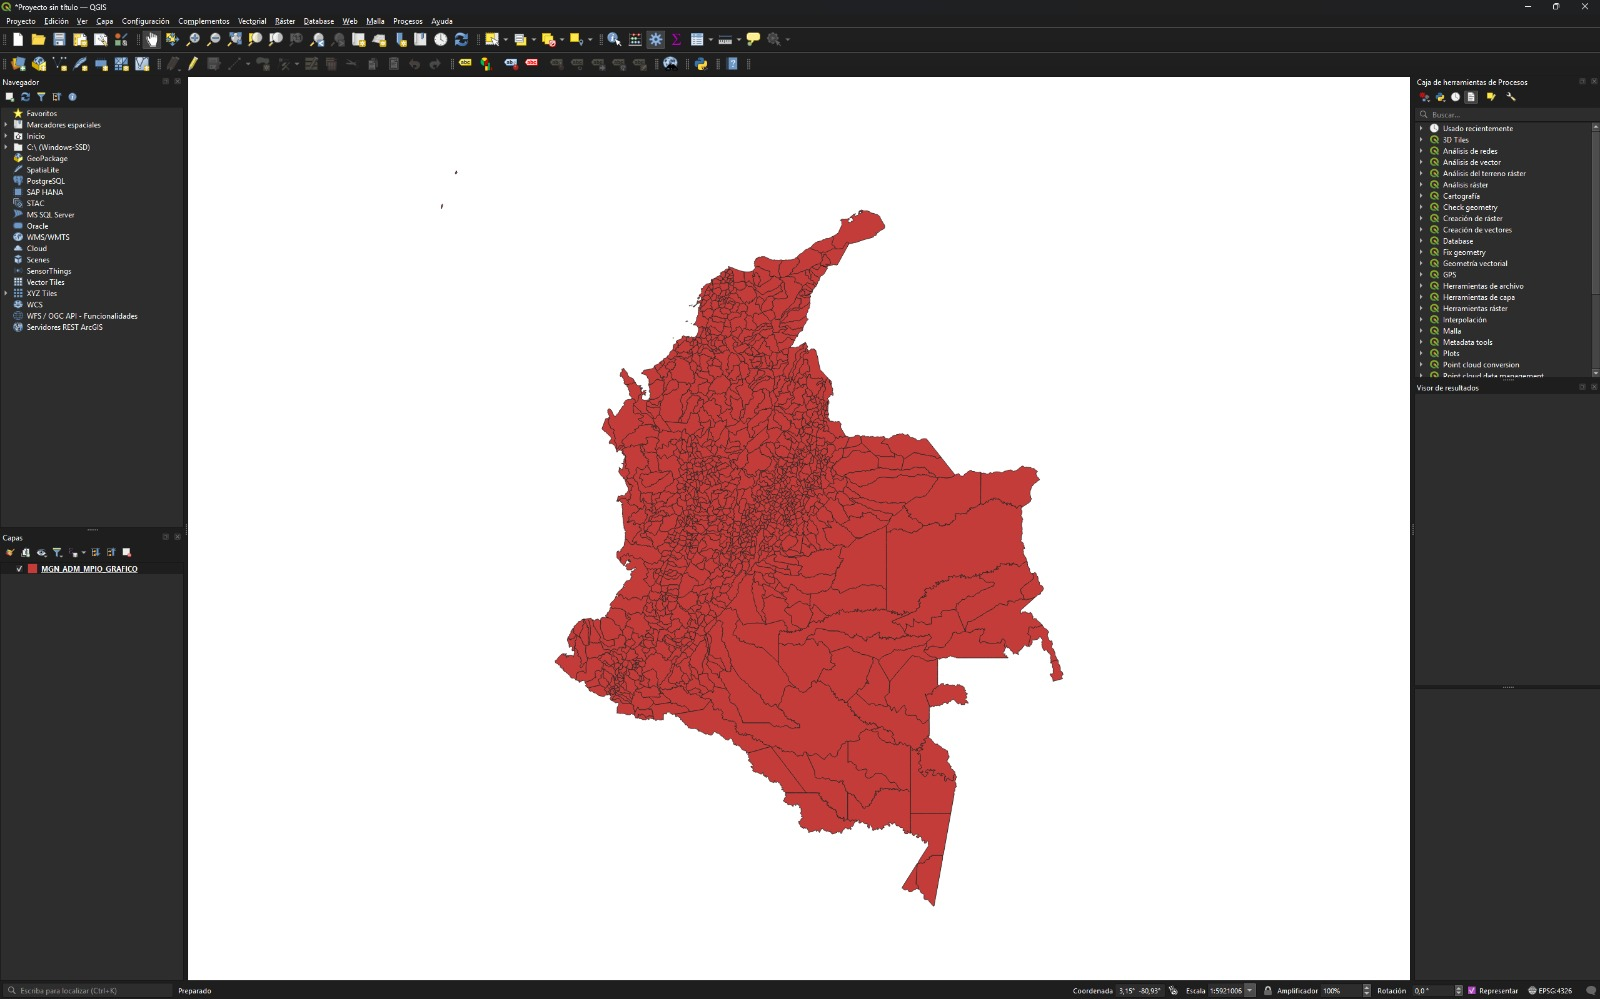
\includegraphics[width=0.95\linewidth]{Imagenes/mgn_shp_qgis.jpeg}
    \caption{Visualización del shapefile administrativo \texttt{MGN\_ADM\_MPIO\_GRAFICO.shp} cargado en QGIS. La capa representa la totalidad de municipios contenidos en el Marco Geoestadístico Nacional (MGN 2025) del DANE.}
    \label{fig:mgn_original}
\end{figure}

Posteriormente, el script en Python realizó el filtrado territorial correspondiente a municipios priorizados PDET y generó el archivo geoespacial:

\begin{center}
\texttt{pdet\_final.geojson}
\end{center}

\begin{figure}[H]
    \centering
    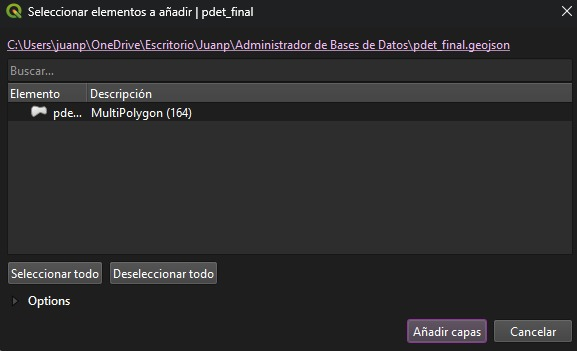
\includegraphics[width=0.72\linewidth]{Imagenes/pdet_python_plot.jpeg}
    \caption{Visualización programática del archivo \texttt{pdet\_final.geojson} generado mediante Python y GeoPandas. Cada color representa municipios PDET filtrados tras el proceso de integración territorial.}
    \label{fig:pdet_geojson}
\end{figure}

Las visualizaciones obtenidas permitieron realizar un proceso preliminar de validación espacial, verificando continuidad topológica y consistencia geométrica respecto al shapefile original del DANE.

\subsubsection{Validación geoespacial y control de calidad}

Con el objetivo de validar la integridad geométrica del dataset resultante, se realizaron pruebas visuales mediante QGIS y validaciones programáticas utilizando Python.

Las validaciones efectuadas incluyeron:

\begin{itemize}
    \item Superposición correcta entre el shapefile original y el GeoJSON generado.
    \item Validación por lotes de geometrías municipales.
    \item Validación individual de polígonos territoriales.
    \item Verificación de continuidad espacial.
    \item Detección de posibles desplazamientos o geometrías corruptas.
\end{itemize}

\vspace{0.3cm}

\textbf{Superposición de capas territoriales}

La superposición entre capas permitió verificar que la transformación espacial no introdujera inconsistencias territoriales ni pérdida de entidades durante la conversión.

\begin{figure}[H]
    \centering
    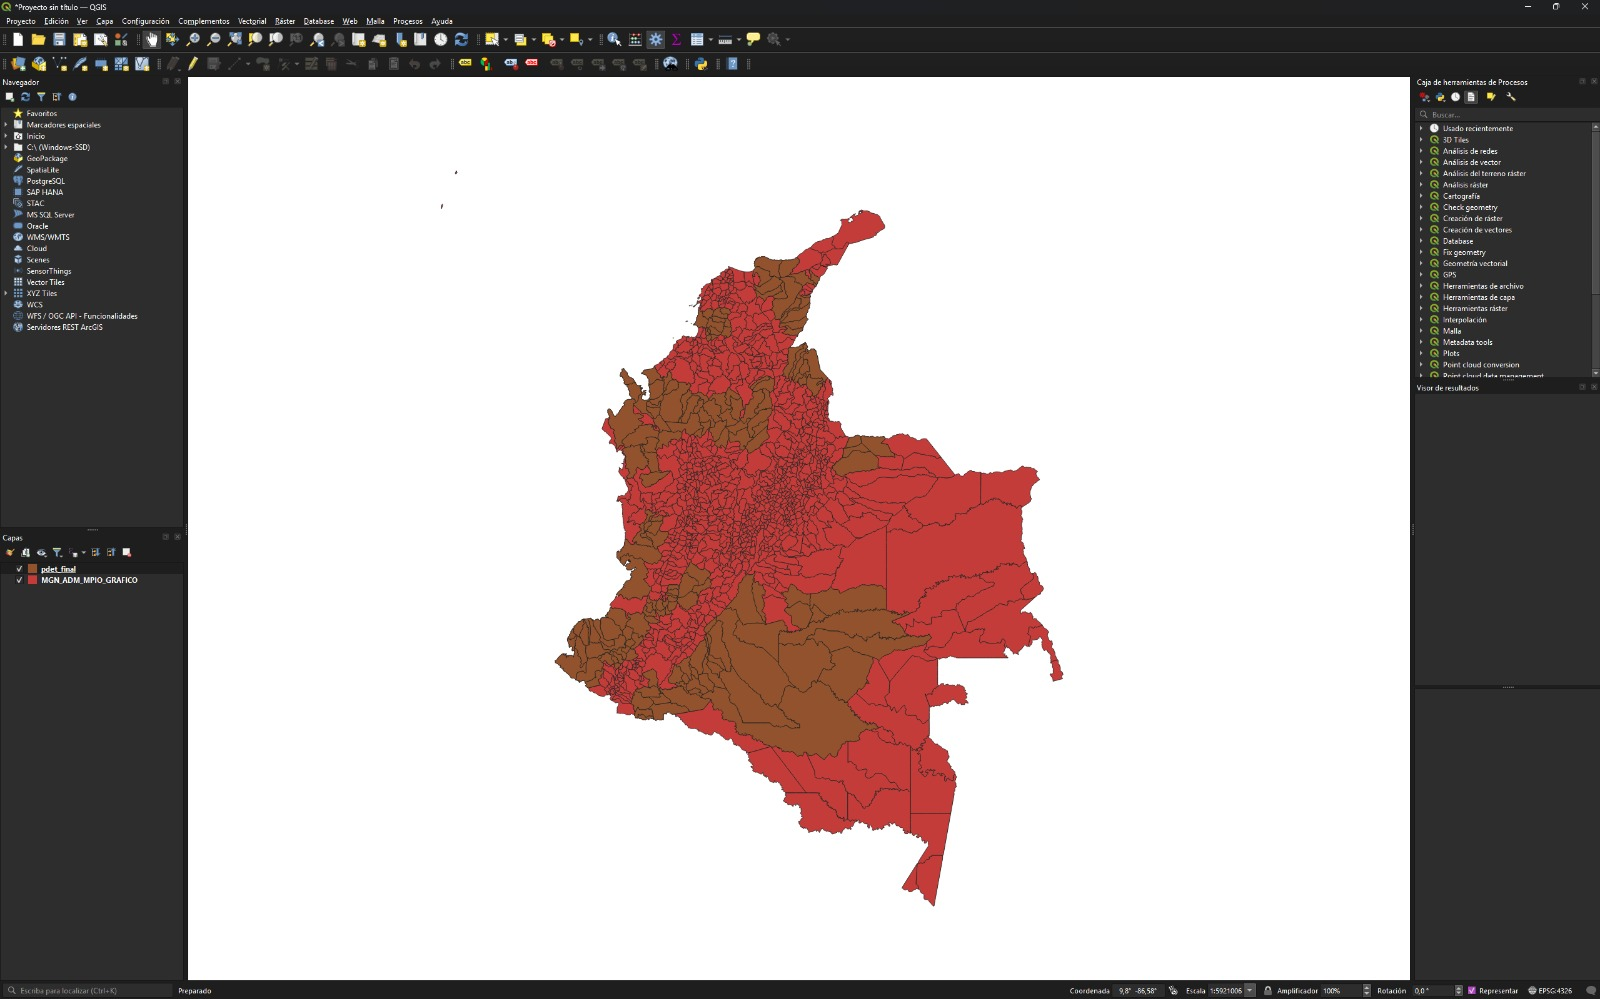
\includegraphics[width=0.92\linewidth]{Imagenes/capas_superpuestas.jpeg}
    \caption{Superposición entre el shapefile original del DANE y el archivo \texttt{pdet\_final.geojson}. La comparación permitió validar continuidad topológica y consistencia espacial entre ambas capas.}
    \label{fig:capas_superpuestas}
\end{figure}

\vspace{0.3cm}

\textbf{Validación visual mediante simbología}

Adicionalmente, se realizaron pruebas manuales modificando simbologías y colores de capas dentro de QGIS con el fin de identificar posibles anomalías geométricas o desplazamientos espaciales.

\begin{figure}[H]
    \centering
    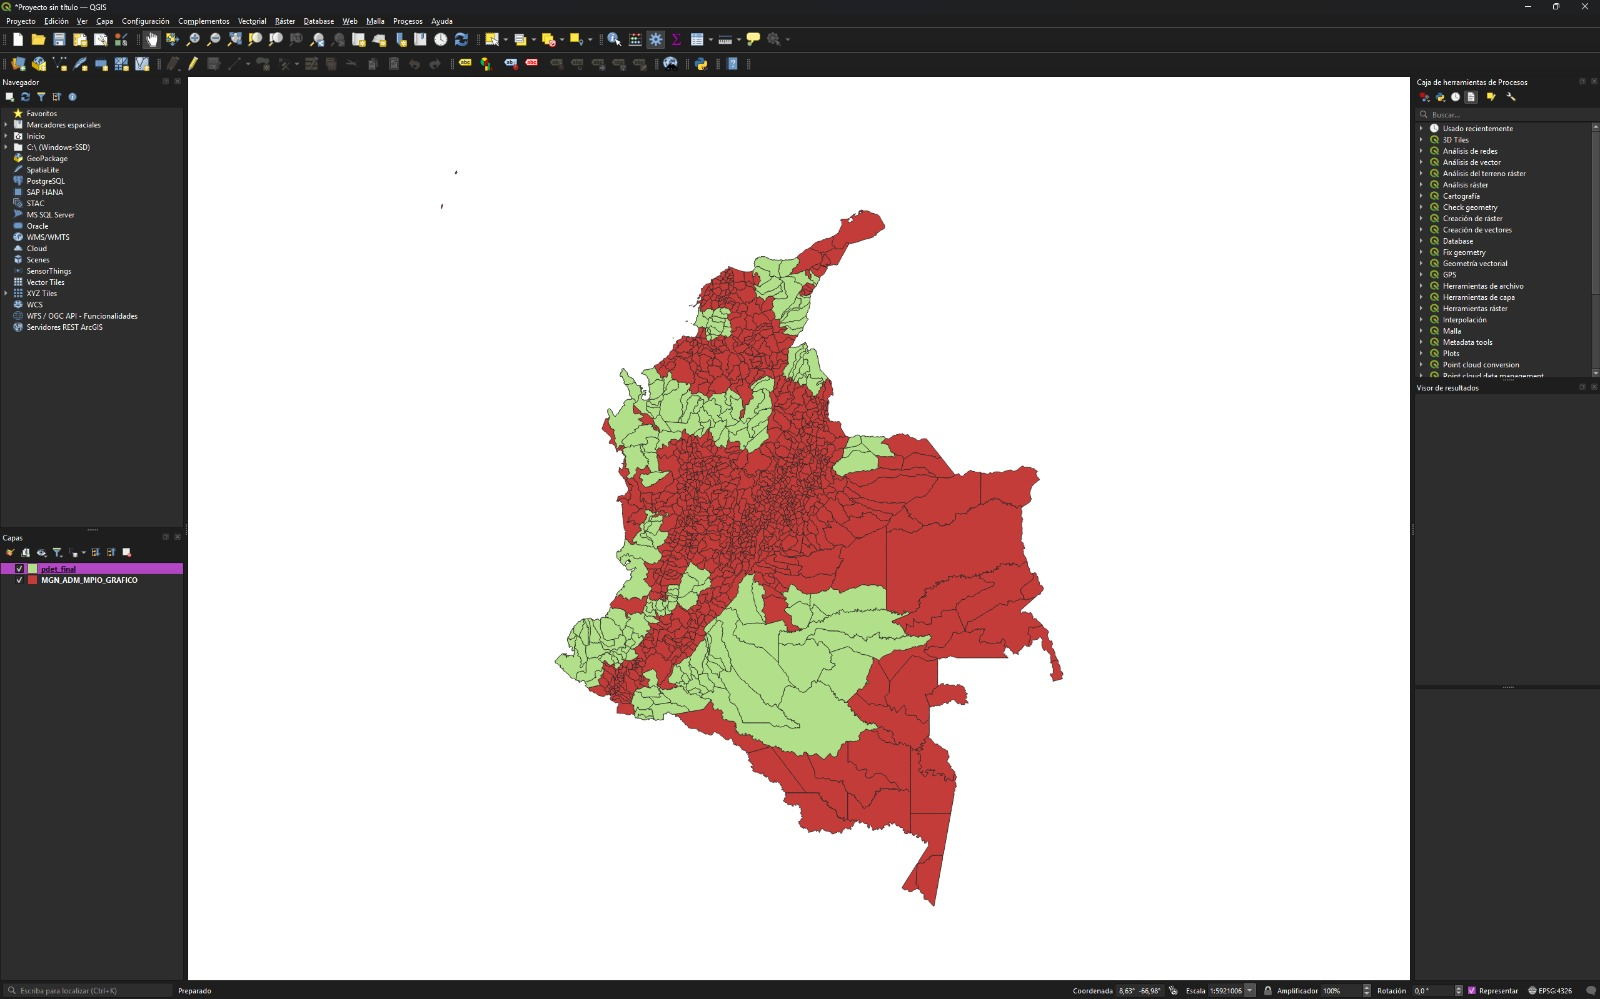
\includegraphics[width=0.92\linewidth]{Imagenes/validacion_colores.jpeg}
    \caption{Validación visual mediante modificación de simbología y colores en QGIS. Este procedimiento permitió identificar posibles inconsistencias geométricas y verificar independencia topológica entre polígonos municipales.}
    \label{fig:validacion_colores}
\end{figure}

\vspace{0.3cm}

\textbf{Validación por lotes}

El proceso de control incluyó validaciones por lotes sobre múltiples geometrías municipales para verificar integridad estructural y correcta carga espacial.

\begin{figure}[H]
    \centering
    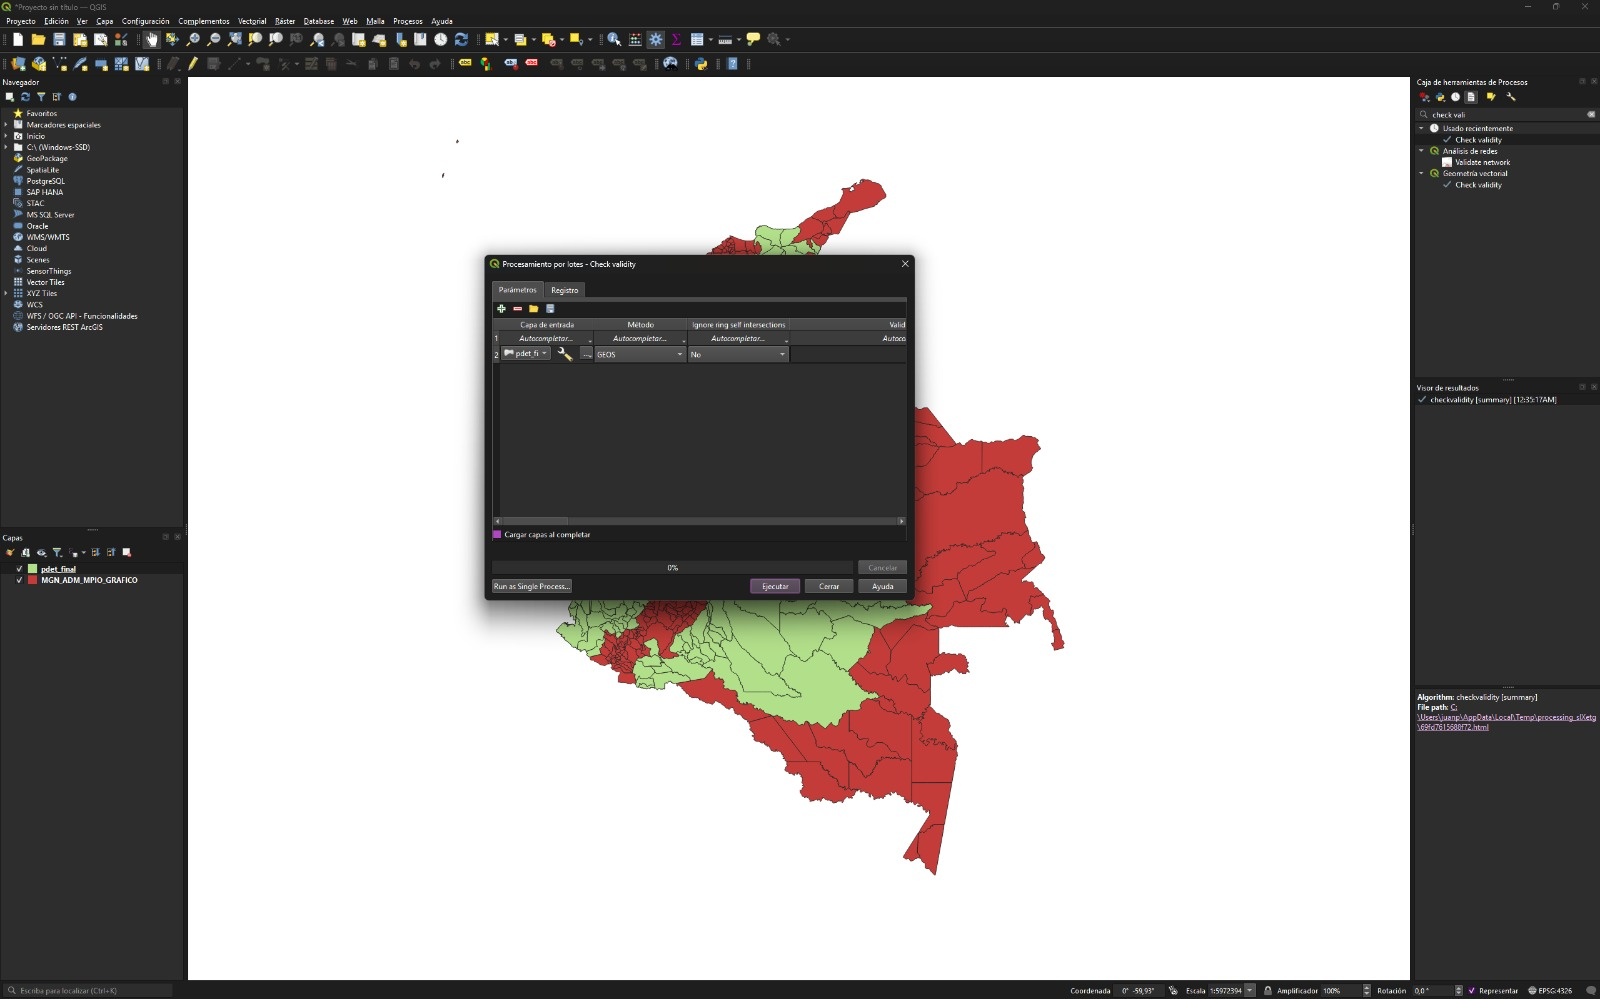
\includegraphics[width=0.82\linewidth]{Imagenes/validacion_lotes.jpeg}
    \caption{Proceso de validación por lotes realizado sobre múltiples geometrías municipales. La validación confirmó una carga espacial exitosa y ausencia de errores topológicos críticos.}
    \label{fig:validacion_lotes}
\end{figure}

\vspace{0.3cm}

\textbf{Validación individual de geometrías}

También se realizaron inspecciones individuales sobre municipios específicos con el objetivo de corroborar la correcta representación cartográfica y creación adecuada de nuevas capas territoriales.

\begin{figure}[H]
    \centering
    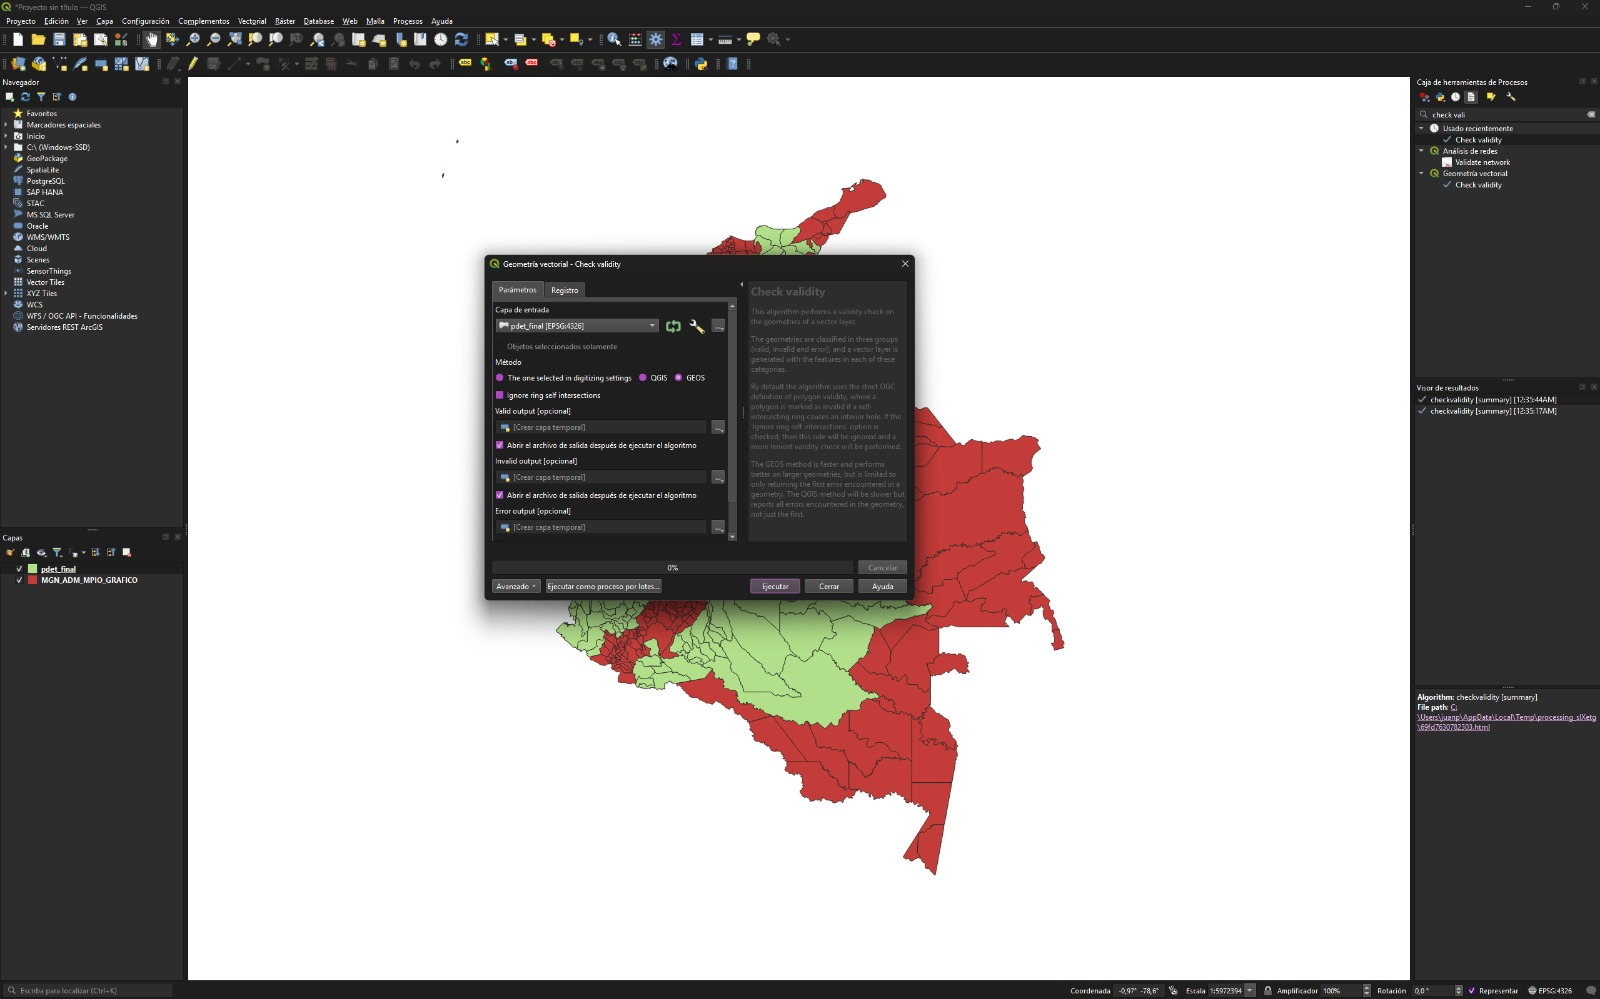
\includegraphics[width=0.82\linewidth]{Imagenes/validacion_individual.jpeg}
    \caption{Validación individual de geometrías territoriales. La inspección permitió corroborar la correcta representación cartográfica de municipios específicos dentro del conjunto PDET.}
    \label{fig:validacion_individual}
\end{figure}

\vspace{0.3cm}

\textbf{Evidencia de ejecución del pipeline}

Durante la ejecución del pipeline geoespacial se obtuvieron resultados de validación en consola similares a los siguientes:

\begin{verbatim}
Cruce por código DANE: encontrados 170 registros.

--- RESULTADOS ---
Municipios cargados del SHP: 1122
Municipios en tu lista PDET: 170
Municipios PDET encontrados tras el cruce: 170

[OK] Archivo 'pdet_final.geojson' creado correctamente.
\end{verbatim}

Estos resultados evidencian la correcta integración territorial y la generación satisfactoria del dataset geoespacial requerido para etapas posteriores del proyecto.

\begin{figure}[H]
    \centering
    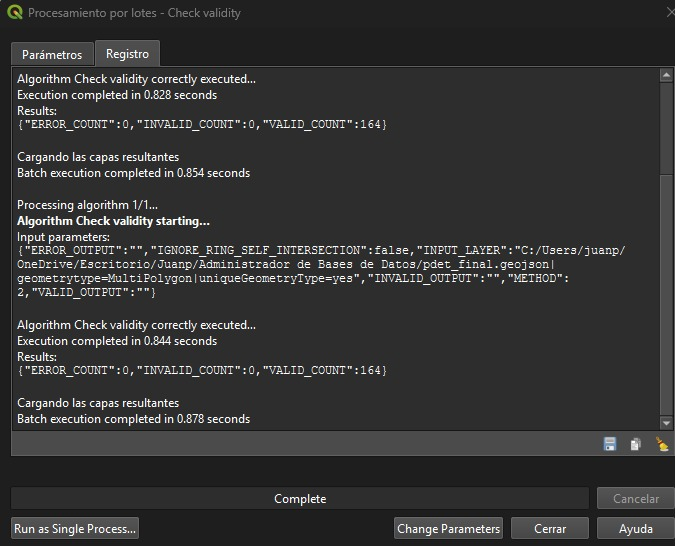
\includegraphics[width=0.95\linewidth]{Imagenes/python_console.jpeg}
    \caption{Salida en consola del pipeline geoespacial implementado en Python, evidenciando la carga del shapefile, integración territorial y generación del archivo GeoJSON final.}
    \label{fig:console_output}
\end{figure}

\vspace{0.3cm}

\textbf{Exportación geoespacial final}

La exportación del subconjunto territorial resultante se realizó mediante la siguiente instrucción:

\begin{verbatim}
resultado_final.to_file(
    "pdet_final.geojson",
    driver="GeoJSON"
)
\end{verbatim}

Esta transformación constituye una etapa crítica dentro del pipeline geoespacial, debido a que permite convertir estructuras territoriales tradicionales en objetos GeoJSON compatibles con MongoDB y operaciones espaciales NoSQL.

\section{Adquisición de Datos}

\subsection{Google Open Buildings}

\subsubsection{Descripción del dataset}

Google Open Buildings es un dataset desarrollado por Google Research que contiene detecciones de edificios derivadas de imágenes satelitales de alta resolución. La versión 3 del dataset cubre Latinoamérica, el Caribe, África, Asia del Sur y Asia del Sureste, con un área de inferencia de 58 millones de km\textsuperscript{2}.

\begin{table}[H]
\centering
\caption{Características del dataset Google Open Buildings}
\begin{tabular}{>{\bfseries}p{5cm} p{8cm}}
\toprule
\tblhdr{Atributo} & \tblhdr{Detalle} \\
\midrule
Versión           & v3 (tercera versión) \\
\rowcolor{grisfilas}
Detecciones totales & $\sim$1.8 mil millones \\
Área de cobertura & 58 millones de km\textsuperscript{2} \\
\rowcolor{grisfilas}
Formato de distribución & CSV comprimido (.csv.gz) por cuadrante \\
Atributos principales & geometry (WKT), area\_in\_meters, confidence, full\_plus\_code \\
\rowcolor{grisfilas}
Licencia          & CC BY-4.0 / ODbL v1.0 \\
URL               & \url{https://sites.research.google/gr/open-buildings/} \\
\bottomrule
\end{tabular}
\end{table}

\subsubsection{Proceso de descarga}

Los archivos fueron descargados directamente desde el portal de Google Open Buildings, filtrando por la región correspondiente a Colombia. Cada archivo CSV comprimido contiene las huellas de edificios para un cuadrante geográfico específico, con los siguientes campos principales:

\begin{figure}[h]
    \centering
    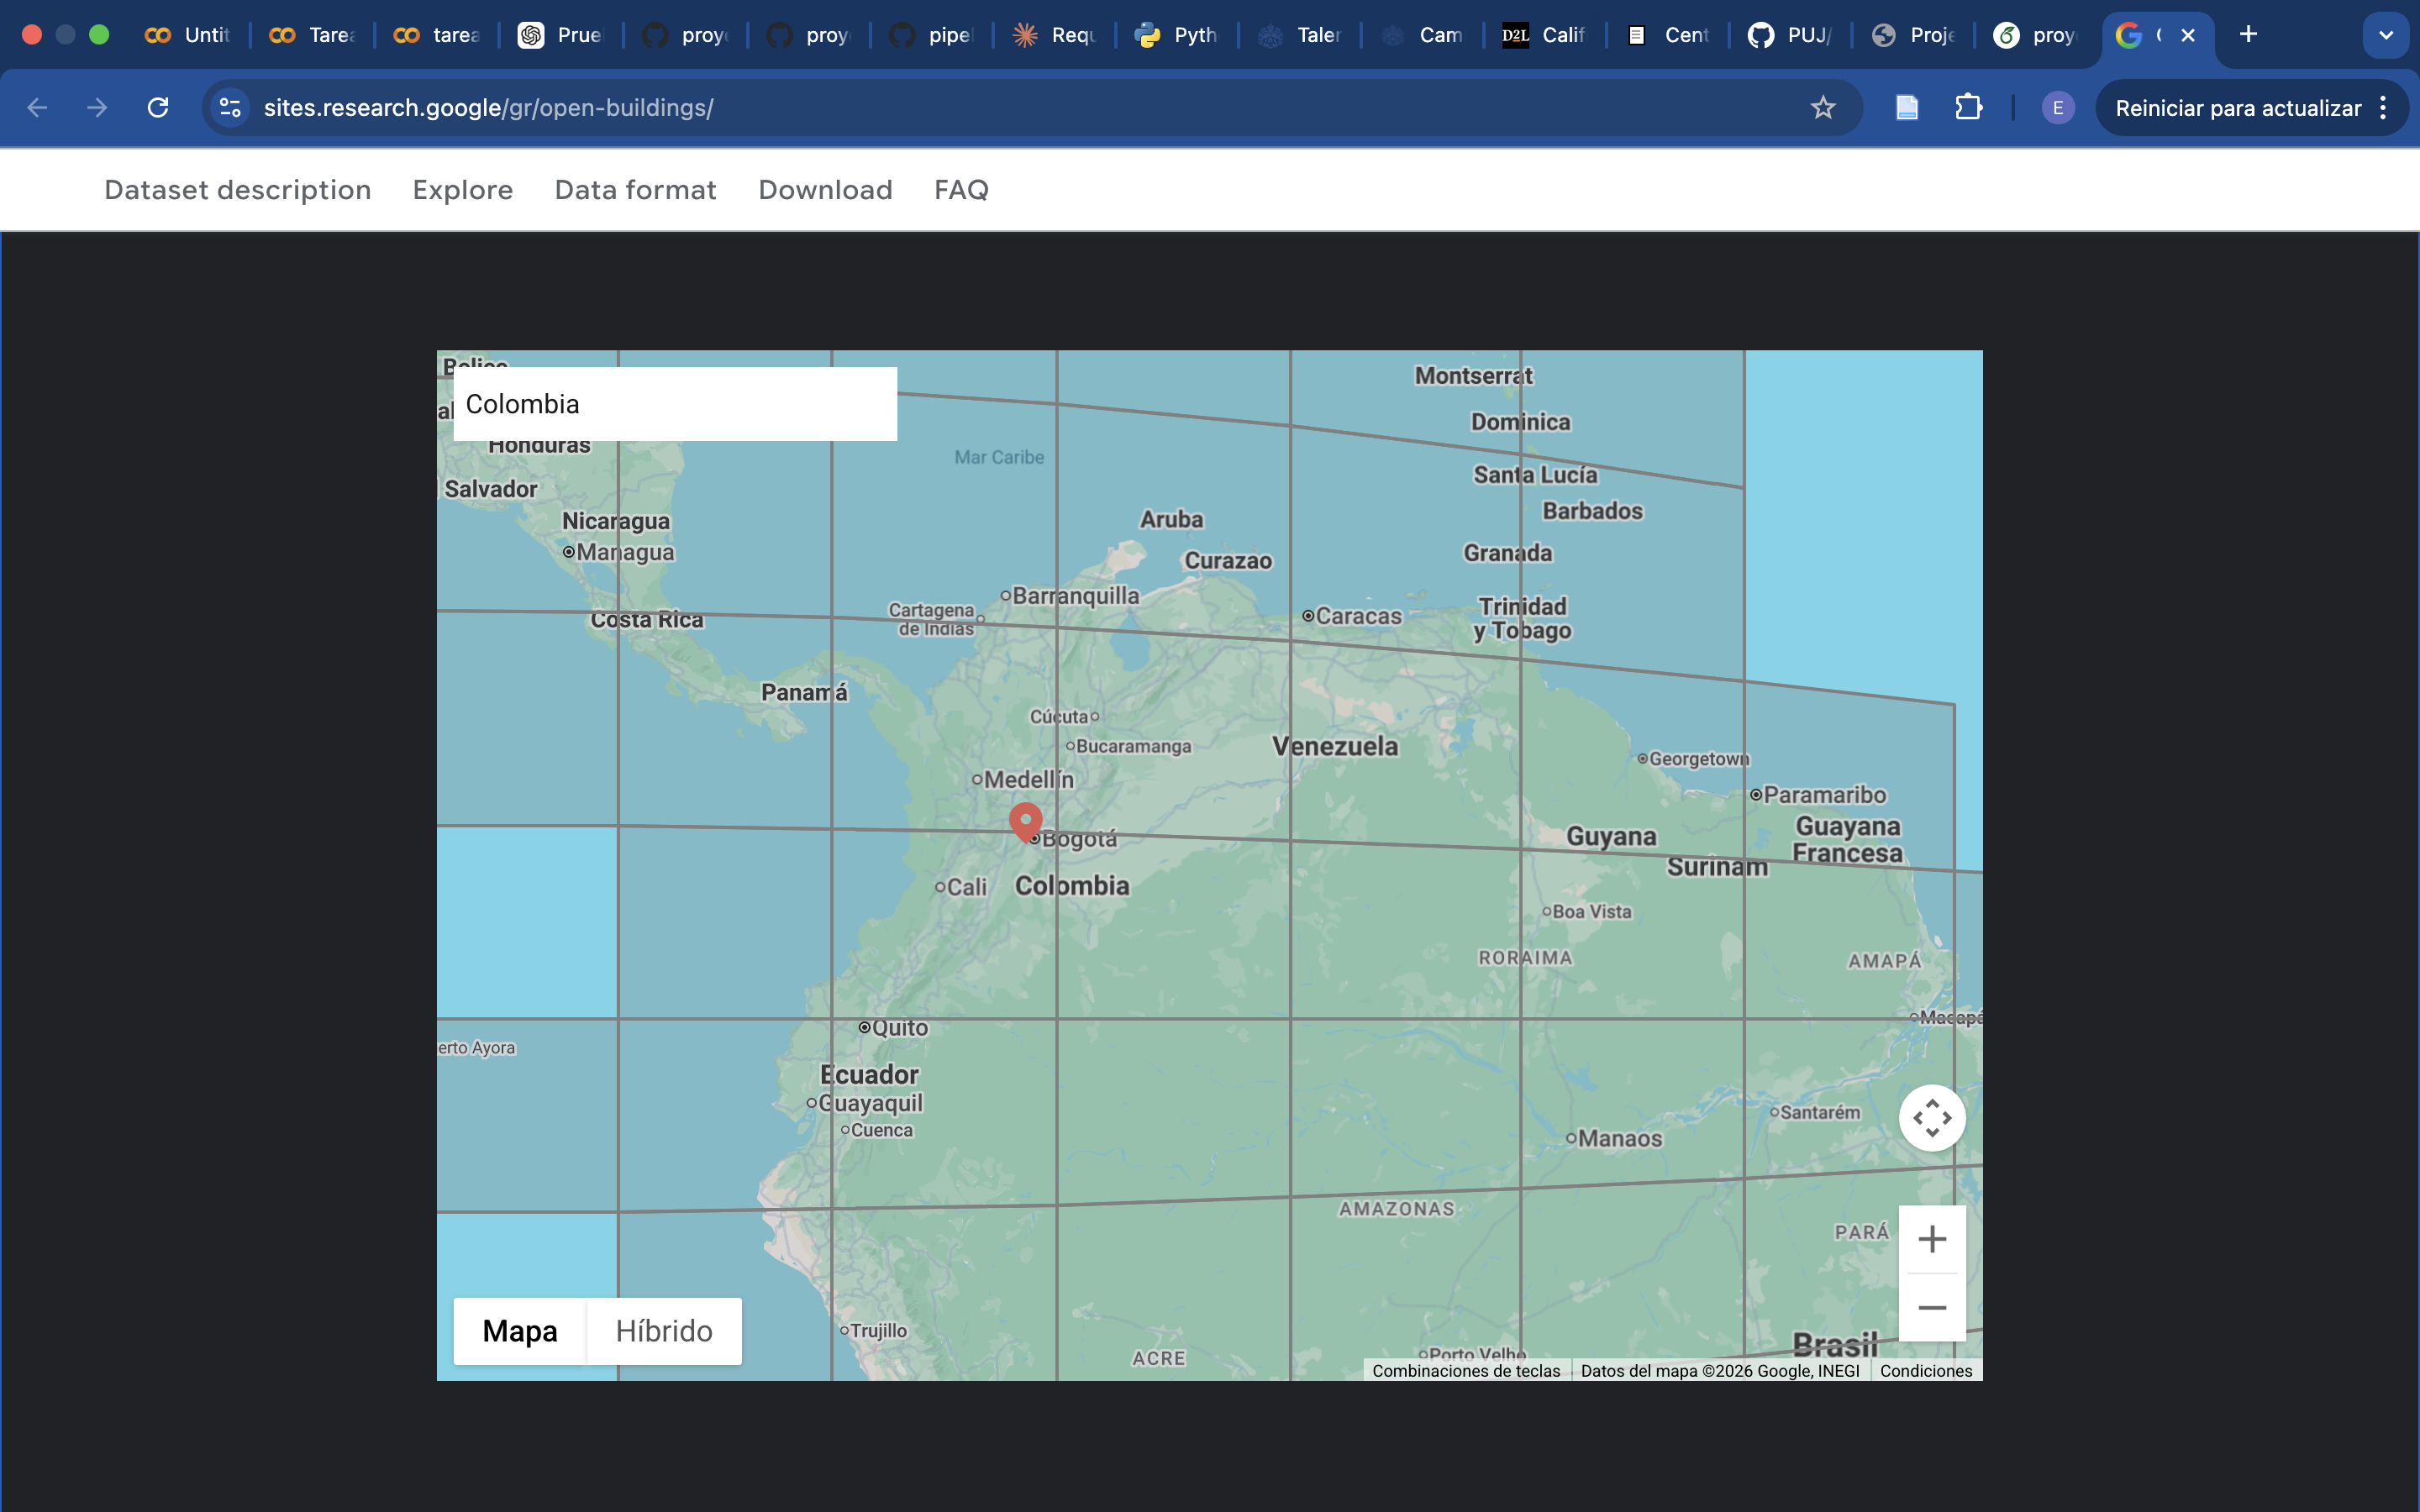
\includegraphics[width=0.5\textwidth]{Imagenes/google.png}
    \caption{Microsoft Building Footprints}
    \label{fig:micro_imagen}
\end{figure}

Esto descarga unos archivos .csv.grz en los cuales estan los datos,en el script.py,se aplicó un filtro mínimo de confianza de \textbf{0.60} durante la carga, descartando detecciones con baja certeza de ser edificaciones reales.

\subsection{Microsoft Global ML Building Footprints}

\subsubsection{Descripción del dataset}

Microsoft Global ML Building Footprints es un dataset desarrollado por Microsoft Research a partir de imágenes de Bing Maps recolectadas entre 2014 y 2021, incorporando fuentes como Maxar y Airbus. Contiene más de 999 millones de detecciones de edificios a nivel mundial.

\begin{table}[H]
\centering
\caption{Características del dataset Microsoft Building Footprints}
\begin{tabular}{>{\bfseries}p{5cm} p{8cm}}
\toprule
\tblhdr{Atributo} & \tblhdr{Detalle} \\
\midrule
Detecciones totales & $>$999 millones \\
\rowcolor{grisfilas}
Período de imágenes & 2014 -- 2021 \\
Formato de distribución & GeoJSON por cuadrante (QuadKey) \\
\rowcolor{grisfilas}
Atributos principales & geometry (GeoJSON Polygon), height, confidence \\
Licencia          & Open Data Commons Open Database License (ODbL) \\
\rowcolor{grisfilas}
URL               & \url{https://planetarycomputer.microsoft.com/dataset/ms-buildings} \\
\bottomrule
\end{tabular}
\end{table}

\subsubsection{Proceso de descarga}

Microsoft distribuye sus datos a través de un índice CSV que lista todos los cuadrantes disponibles por país. El proceso de descarga se basó en el snippet oficial de Microsoft, adaptado para filtrar únicamente los cuadrantes correspondientes a Colombia,este proceso se descarga se puede ver en el pruebasDosMicro.py:

\begin{figure}[h]
    \centering
    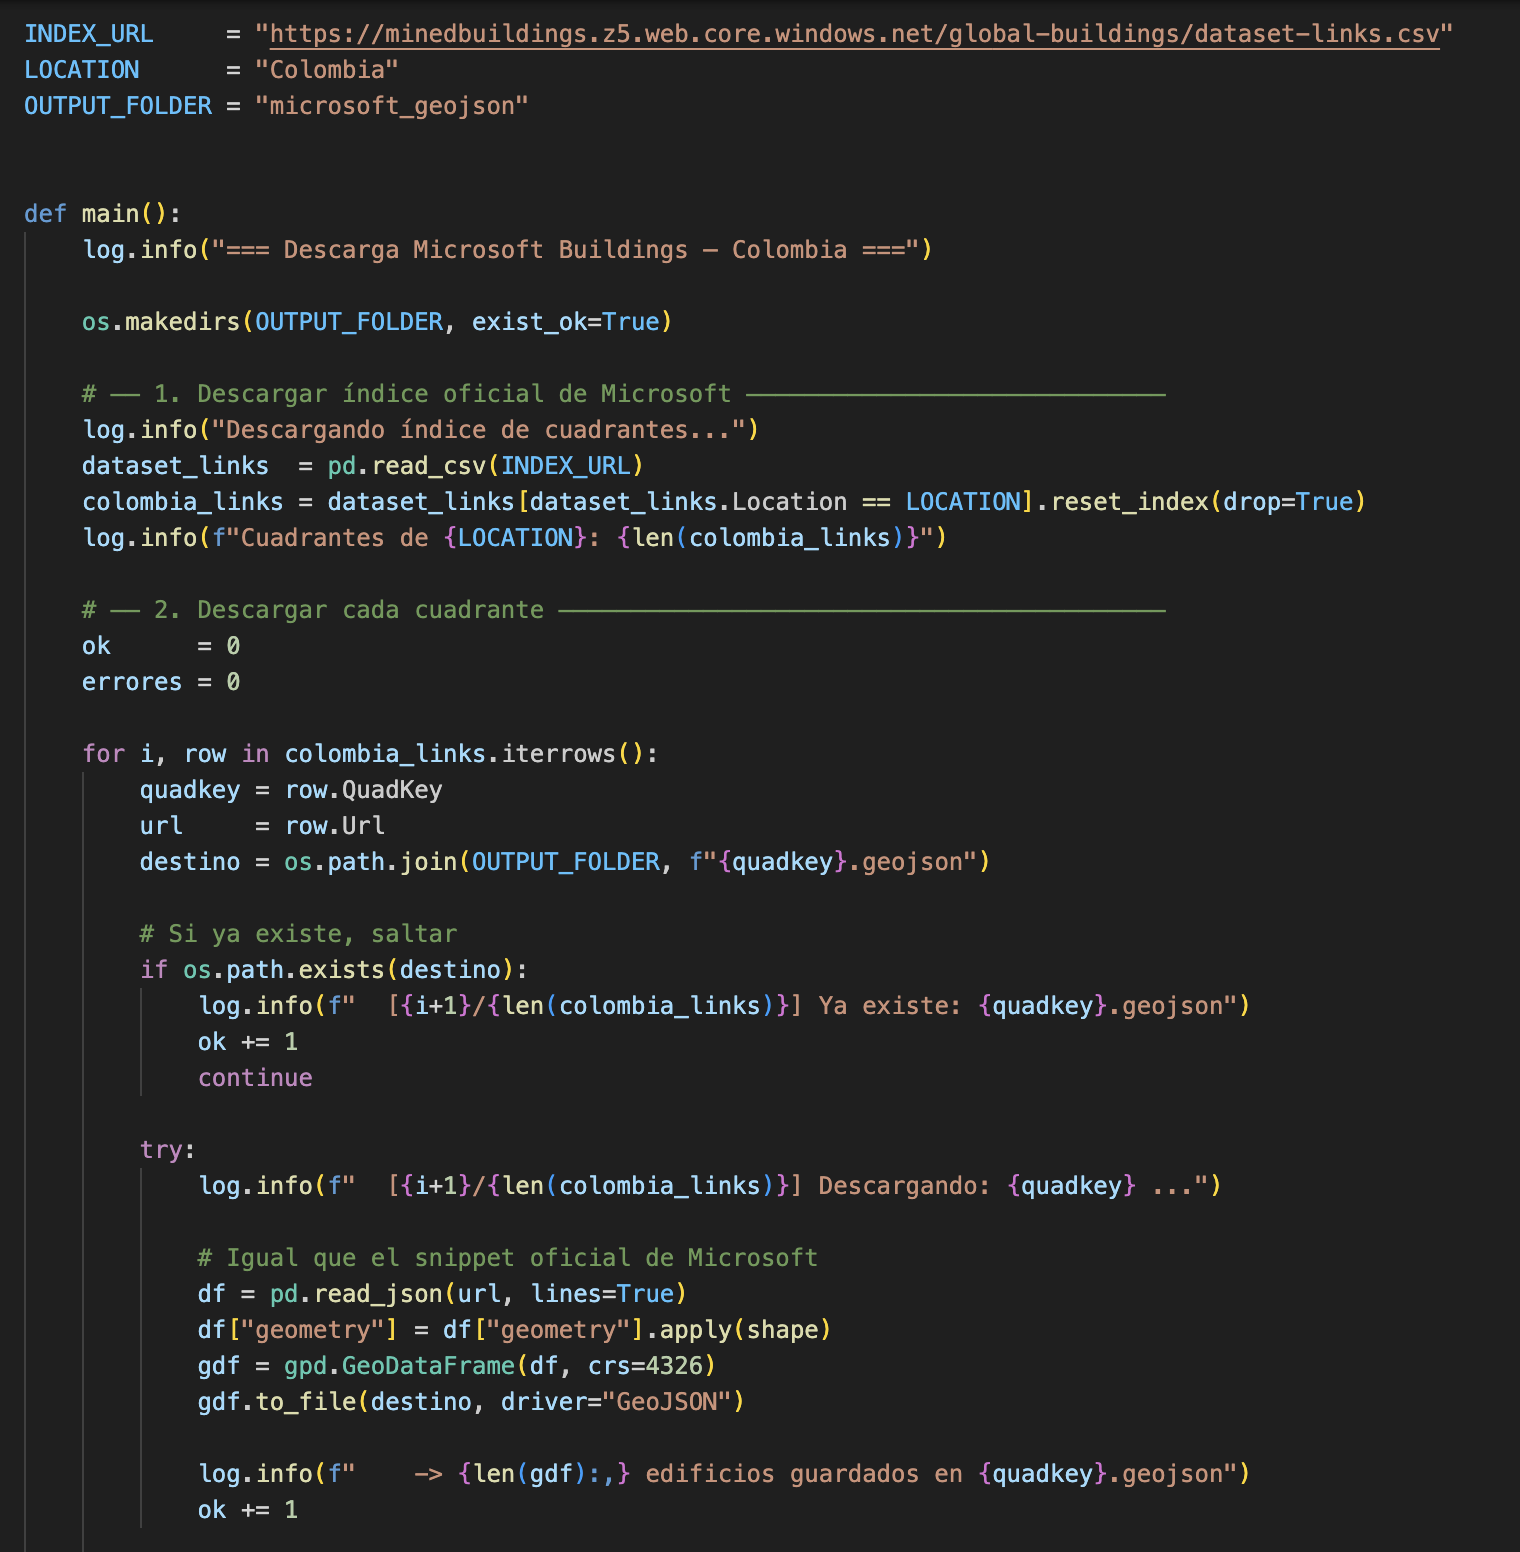
\includegraphics[width=0.5\textwidth]{Imagenes/micro.png}
    \caption{Google open buildings}
    \label{fig:mi_imagen}
\end{figure}

Para Colombia se identificaron y descargaron \textbf{229 cuadrantes GeoJSON}, cada uno correspondiente a un QuadKey único del sistema de indexación de Bing Maps.

% ══════════════════════════════════════════════════════════════════════════════
\section{Integración en MongoDB e Indexación Espacial}

\subsection{Arquitectura de colecciones}

Los datos fueron almacenados en tres colecciones dentro de la base de datos \texttt{proyecto} en MongoDB:

\begin{table}[H]
\centering
\caption{Colecciones en MongoDB}
\begin{tabular}{p{4.5cm} p{3cm} p{5cm}}
\toprule
\tblhdr{Colección} & \tblhdr{Documentos} & \tblhdr{Propósito} \\
\midrule
\texttt{territorios\_pdet}   & 170         & Límites municipales PDET \\
\rowcolor{grisfilas}
\texttt{google\_buildings}   & 2,687,624   & Huellas de edificios (Google) \\
\texttt{microsoft\_buildings} & 1,537,635  & Huellas de edificios (Microsoft) \\
\bottomrule
\end{tabular}
\end{table}

\subsection{Esquema de documento}

Cada edificio, independientemente de la fuente, sigue el esquema unificado definido desde la semana 1:

\begin{lstlisting}[language=JavaScript, caption={Esquema unificado de documento en mongodb}]
{
  "_id":              ObjectId,
  "fuente":           "google" | "microsoft",
  "codigo_mgn":       "47001",          // codigo DANE del municipio
  "nombre_municipio": "SANTA MARTA",
  "geometria_edificio": {               // GeoJSON Polygon
    "type": "Polygon",
    "coordinates": [[[lng, lat], ...]]
  },
  "area_estimada_m2": 87.39,            // solo Google
  "metadata": {
    "confianza":       0.78,
    "altura_m":        null,            // solo Microsoft cuando disponible
    "fuente_imagen":   "Google Satellite Imagery",
    "dataset_version": "Google Open Buildings v3"
  }
}
\end{lstlisting}

\subsection{Indexación espacial}

Se implementaron índices \texttt{2dsphere} sobre el campo \texttt{geometria\_edificio} en ambas colecciones de edificios, junto con índices auxiliares para acelerar consultas por fuente y municipio:

\begin{lstlisting}[language=Python, caption={Creación de índices espaciales en MongoDB}]
# Indice geoespacial 2dsphere (requerido para geoWithin, geoIntersects)
col.create_index(
    [("geometria_edificio", GEOSPHERE)],
    name="idx_geo_edificio"
)
# Indices auxiliares para agregaciones
col.create_index("fuente",     name="idx_fuente")
col.create_index("codigo_mgn", name="idx_codigo_mgn")
\end{lstlisting}

\subsection{Proceso de cruce espacial y filtro PDET}

Un paso crítico en el pipeline de carga fue el cruce espacial entre cada edificio y los polígonos PDET. Solo se insertaron en MongoDB los edificios cuyo centroide cayera \textit{dentro} de algún municipio PDET. Este filtro se implementó de dos formas según la fuente:

\begin{itemize}[leftmargin=1.5cm]
    \item \textbf{Google}: lectura por lotes de archivos CSV, conversión de geometrías WKT a objetos Shapely, uso de \texttt{STRtree} para consulta espacial eficiente y validación mediante el centroide de cada huella contra los polígonos PDET.
    \item \textbf{Microsoft}: lectura de archivos GeoJSON por cuadrante, reparación y validación de geometrías poligonales, asignación municipal mediante el centroide de cada edificio y limpieza posterior de geometrías incompatibles con índices \texttt{2dsphere}.
\end{itemize}

Aunque MongoDB permite ejecutar consultas espaciales mediante operadores como \texttt{\$geoWithin} y \texttt{\$geoIntersects}, en el pipeline final se decidió almacenar el campo \texttt{codigo\_mgn} directamente en cada edificio durante la carga. Esta decisión reduce el costo de las agregaciones posteriores, ya que evita repetir cruces espaciales sobre millones de geometrías en cada consulta.

\subsection{Eficiencia de carga}

Para garantizar una carga eficiente de grandes volúmenes de datos, se implementó escritura por lotes con un tamaño de lote de 20,000 documentos. Además, los índices espaciales fueron creados al final de la carga para evitar que MongoDB actualizara los índices durante cada inserción masiva.

\begin{lstlisting}[language=Python, caption={Inserción por lotes optimizada}]
BATCH_SIZE = 20_000

batch.append(doc)

if len(batch) >= BATCH_SIZE:
    col.insert_many(batch, ordered=False)
    batch = []

if batch:
    col.insert_many(batch, ordered=False)
\end{lstlisting}

El parámetro \texttt{ordered=False} permite que MongoDB procese las inserciones en paralelo, mejorando el rendimiento y tolerando errores individuales sin detener el proceso completo.

\section{Auditoría Inicial de Datos (EDA)}

\subsection{Resumen general}

Tras completar la carga de ambos datasets, se realizó un análisis exploratorio de datos (EDA) directamente sobre las colecciones de MongoDB mediante pipelines de agregación. Los resultados globales se presentan a continuación:

\begin{table}[H]
\centering
\caption{Resumen general de edificios cargados y consolidación final}
\begin{tabular}{p{8cm} r}
\toprule
\tblhdr{Métrica} & \tblhdr{Valor} \\
\midrule
Municipios PDET cargados & 170 \\
\rowcolor{grisfilas}
Edificios Google cargados & 2.687.624 \\
Edificios Microsoft cargados después de limpieza geométrica & 1.537.635 \\
\rowcolor{grisfilas}
Total de huellas procesadas en ambas fuentes & 4.225.259 \\
Duplicados Microsoft-Google detectados & 764.492 \\
\rowcolor{grisfilas}
Edificios Microsoft únicos agregados & 773.143 \\
Total final de edificios sin duplicados & \textbf{3.460.767} \\
\rowcolor{grisfilas}
Área total de techos sin duplicados (m\textsuperscript{2}) & 
\textbf{282.191.579,71} \\
Área total de techos sin duplicados (ha) & 28.219,16 \\
Área total de techos sin duplicados (km\textsuperscript{2}) & 282,19 \\
\bottomrule
\end{tabular}
\end{table}

\textbf{Nota sobre Microsoft}: el dataset de Microsoft no incluye el campo \texttt{area\_in\_meters} en sus GeoJSON de distribución. Los valores de \texttt{height} y \texttt{confidence} registrados en los archivos descargados para Colombia presentaron valores de \texttt{-1}, indicando que no estaban disponibles para esta región en particular.

Debido a la ausencia de un atributo de área directamente comparable en Microsoft, el área de techos para esta fuente fue calculada geométricamente a partir de las huellas proyectadas al sistema de referencia métrico \texttt{EPSG:9377}. Para mantener consistencia metodológica, el análisis final también calculó áreas geométricas sobre las huellas consolidadas.

\subsection{Cobertura territorial comparativa}

La cobertura territorial se evaluó sobre los \textbf{170 municipios PDET} cargados en la colección \texttt{territorios\_pdet}. Para cada municipio se calcularon conteos separados por fuente y un resultado consolidado sin duplicados.

La estrategia final no consistió únicamente en sumar las detecciones de Google y Microsoft. En cambio, se compararon espacialmente las huellas de ambas fuentes para identificar posibles duplicados. Cuando una huella de Microsoft presentaba un solapamiento significativo con una huella de Google, se consideró duplicada y no se agregó al resultado final.

La regla de deduplicación utilizada fue:

\[
\frac{\text{Área de intersección}}{\min(\text{Área Google}, \text{Área Microsoft})} \geq 0.50
\]

Bajo esta regla, Google se conservó como fuente prioritaria y Microsoft se utilizó como fuente complementaria para agregar únicamente edificios no detectados por Google.

\begin{table}[H]
\centering
\caption{Consolidación entre fuentes después de deduplicación espacial}
\begin{tabular}{p{8cm} r}
\toprule
\tblhdr{Categoría} & \tblhdr{Edificios} \\
\midrule
Google Open Buildings & 2.687.624 \\
\rowcolor{grisfilas}
Microsoft Building Footprints original & 1.537.635 \\
Duplicados Microsoft-Google & 764.492 \\
\rowcolor{grisfilas}
Microsoft únicos agregados & 773.143 \\
\textbf{Total final sin duplicados} & \textbf{3.460.767} \\
\bottomrule
\end{tabular}
\end{table}

\subsection{Top 20 municipios por número de edificios — Google Open Buildings}

\begin{longtable}{r l r r r}
\caption{Top 20 municipios PDET por número de edificios (Google, versión final)} \\
\toprule
\tblhdr{\#} & \tblhdr{Municipio} & \tblhdr{Edificios} & \tblhdr{Área Total (m\textsuperscript{2})} & \tblhdr{Área Prom. (m\textsuperscript{2})} \\
\midrule
\endfirsthead
\toprule
\tblhdr{\#} & \tblhdr{Municipio} & \tblhdr{Edificios} & \tblhdr{Área Total (m\textsuperscript{2})} & \tblhdr{Área Prom. (m\textsuperscript{2})} \\
\midrule
\endhead
\bottomrule
\endfoot
1  & SANTA MARTA              & 183,652 & 15,966,845.25 & 86.94 \\
\rowcolor{grisfilas}
2  & VALLEDUPAR               & 171,425 & 15,306,269.53 & 89.29 \\
3  & BUENAVENTURA             & 103,890 & 7,658,352.05  & 73.72 \\
\rowcolor{grisfilas}
4  & TURBO                    & 78,927  & 6,036,411.11  & 76.48 \\
5  & FLORENCIA                & 58,135  & 7,334,010.74  & 126.15 \\
\rowcolor{grisfilas}
6  & SAN ANDRES DE TUMACO     & 50,493  & 3,793,315.73  & 75.13 \\
7  & TIERRALTA                & 43,123  & 3,078,702.71  & 71.39 \\
\rowcolor{grisfilas}
8  & CIENAGA                  & 42,068  & 3,955,667.01  & 94.03 \\
9  & CAJIBIO                  & 41,281  & 2,573,777.82  & 62.35 \\
\rowcolor{grisfilas}
10 & EL TAMBO                 & 38,900  & 2,449,152.18  & 62.96 \\
11 & EL CARMEN DE BOLIVAR     & 38,386  & 2,541,160.53  & 66.20 \\
\rowcolor{grisfilas}
12 & APARTADO                 & 36,337  & 3,599,828.36  & 99.07 \\
13 & TAME                     & 35,958  & 3,183,325.12  & 88.53 \\
\rowcolor{grisfilas}
14 & SANTANDER DE QUILICHAO   & 35,691  & 3,842,935.10  & 107.67 \\
15 & ARAUQUITA                & 35,077  & 2,919,565.44  & 83.23 \\
\rowcolor{grisfilas}
16 & AGUSTIN CODAZZI          & 34,733  & 2,699,284.28  & 77.72 \\
17 & TIBU                     & 32,843  & 2,636,703.11  & 80.28 \\
\rowcolor{grisfilas}
18 & SAN JOSE DEL GUAVIARE    & 32,695  & 3,147,419.35  & 96.27 \\
19 & NECOCLI                  & 32,183  & 2,340,769.38  & 72.73 \\
\rowcolor{grisfilas}
20 & MORALES                  & 31,057  & 1,965,301.82  & 63.28 \\
\end{longtable}

\subsection{Top 20 municipios por número de edificios — Microsoft Building Footprints}

\begin{longtable}{r l r r}
\caption{Top 20 municipios PDET por número de edificios (Microsoft, versión final)} \\
\toprule
\tblhdr{\#} & \tblhdr{Municipio} & \tblhdr{Edificios} & \tblhdr{Área Total (m\textsuperscript{2})} \\
\midrule
\endfirsthead
\toprule
\tblhdr{\#} & \tblhdr{Municipio} & \tblhdr{Edificios} & \tblhdr{Área Total (m\textsuperscript{2})} \\
\midrule
\endhead
\bottomrule
\endfoot
1  & SANTA MARTA              & 67,663 & 14,207,992.34 \\
\rowcolor{grisfilas}
2  & SAN ANDRES DE TUMACO     & 41,423 & 4,524,735.40 \\
3  & TIBU                     & 35,478 & 3,569,509.95 \\
\rowcolor{grisfilas}
4  & EL TAMBO                 & 34,366 & 3,051,941.00 \\
5  & BUENAVENTURA             & 33,020 & 7,138,217.08 \\
\rowcolor{grisfilas}
6  & SANTANDER DE QUILICHAO   & 30,841 & 4,234,663.51 \\
7  & TURBO                    & 28,240 & 3,189,172.78 \\
\rowcolor{grisfilas}
8  & ARAUQUITA                & 27,815 & 3,317,209.87 \\
9  & FLORENCIA                & 26,896 & 6,683,829.91 \\
\rowcolor{grisfilas}
10 & EL CARMEN DE BOLIVAR     & 24,235 & 2,189,240.20 \\
11 & CAJIBIO                  & 23,771 & 2,270,334.69 \\
\rowcolor{grisfilas}
12 & SAN VICENTE DEL CAGUAN   & 23,587 & 3,756,489.48 \\
13 & CIENAGA                  & 21,990 & 3,473,952.89 \\
\rowcolor{grisfilas}
14 & SAN JOSE DEL GUAVIARE    & 21,446 & 3,099,880.81 \\
15 & PUERTO ASIS              & 21,234 & 3,056,417.43 \\
\rowcolor{grisfilas}
16 & TAME                     & 20,958 & 2,761,029.83 \\
17 & MONTELIBANO              & 18,723 & 2,498,713.98 \\
\rowcolor{grisfilas}
18 & ORITO                    & 17,840 & 2,029,245.49 \\
19 & SAN ONOFRE               & 17,348 & 1,490,877.96 \\
\rowcolor{grisfilas}
20 & CHAPARRAL                & 16,849 & 1,974,276.54 \\
\end{longtable}

\subsection{Análisis comparativo entre fuentes}

Para los 168 municipios con cobertura en ambas fuentes, se calculó la diferencia en el número de edificios detectados y el ratio Google/Microsoft:

\begin{table}[H]
\centering
\caption{Comparativa de detecciones en municipios con cobertura en ambas fuentes (muestra top 10)}
\begin{tabular}{l r r r r}
\toprule
\tblhdr{Municipio} & \tblhdr{Google} & \tblhdr{Microsoft} & \tblhdr{Diferencia} & \tblhdr{Ratio G/M} \\
\midrule
VALLEDUPAR               & 171,425 & 14,969 & +156,456 & 11.45 \\
\rowcolor{grisfilas}
SANTA MARTA              & 183,652 & 67,663 & +115,989 & 2.71 \\
BUENAVENTURA             & 103,890 & 33,020 & +70,870  & 3.15 \\
\rowcolor{grisfilas}
TURBO                    & 78,927  & 28,240 & +50,687  & 2.79 \\
TIERRALTA                & 43,123  & 4,190  & +38,933  & 10.29 \\
\rowcolor{grisfilas}
APARTADO                 & 36,337  & 2,652  & +33,685  & 13.70 \\
AGUSTIN CODAZZI          & 34,733  & 2,575  & +32,158  & 13.49 \\
\rowcolor{grisfilas}
FLORENCIA                & 58,135  & 26,896 & +31,239  & 2.16 \\
NECOCLI                  & 32,183  & 10,119 & +22,064  & 3.18 \\
\rowcolor{grisfilas}
CIENAGA                  & 42,068  & 21,990 & +20,078  & 1.91 \\
\bottomrule
\end{tabular}
\end{table}

\subsubsection{Hallazgos del análisis comparativo}

\begin{itemize}[leftmargin=1.5cm]
    \item En \textbf{131 de los 168 municipios} comunes, Google detectó más edificios que Microsoft. La razón Google/Microsoft presenta una mediana cercana a \textbf{1.42x}.
    \item En municipios como \textbf{Valledupar} (ratio 11.45x) y \textbf{Tierralta} (ratio 10.29x), la diferencia es pronunciada, lo cual puede explicarse por diferencias en cobertura de imágenes, fechas de captura y criterios de detección entre fuentes.
    \item En \textbf{36 municipios}, Microsoft supera a Google (por ejemplo \textbf{Ataco}, \textbf{López} y \textbf{Rioblanco}), lo que evidencia que Microsoft aporta detecciones únicas en zonas donde Google presenta menor cobertura o mayor subdetección.
    \item La consolidación final no se basa en elegir una única fuente, sino en \textbf{deduplicar espacialmente} y conservar Google como fuente prioritaria, agregando únicamente huellas de Microsoft no solapadas significativamente.
\end{itemize}

\subsection{Observaciones sobre calidad de datos}

\begin{table}[H]
\centering
\caption{Comparación de atributos disponibles por fuente}
\begin{tabular}{p{5cm} c c}
\toprule
\tblhdr{Atributo} & \tblhdr{Google} & \tblhdr{Microsoft} \\
\midrule
Geometría (Polygon)         & \checkmark & \checkmark \\
\rowcolor{grisfilas}
Área estimada (m\textsuperscript{2}) & \checkmark & \texttimes \\
Nivel de confianza          & \checkmark & \texttimes* \\
\rowcolor{grisfilas}
Altura del edificio         & \texttimes & \texttimes* \\
Código de ubicación (Plus Code) & \checkmark & \texttimes \\
\rowcolor{grisfilas}
Municipios PDET analizados   & 170    & 170 \\
Total edificios cargados     & 2,686,933  & 1,537,288 \\
\bottomrule
\multicolumn{3}{l}{\small * Los campos height y confidence de Microsoft aparecen como -1 para Colombia.}
\end{tabular}
\end{table}



% ══════════════════════════════════════════════════════════════════════════════
\section{Análisis Reproducible de Rooftops y Generación de Resultados}

\subsection{Objetivo del análisis}

Con el fin de consolidar una metodología reproducible para el análisis del potencial solar en municipios PDET, se desarrolló el script:

\begin{center}
\texttt{02\_rooftop\_analysis.py}
\end{center}

Este componente automatiza el cálculo de:

\begin{itemize}
    \item Conteo total de edificaciones por municipio.
    \item Área total estimada de techos.
    \item Métricas de calidad espacial.
    \item Exportación geoespacial en formato GeoJSON.
    \item Generación automática de mapas temáticos.
\end{itemize}

El análisis se ejecuta directamente sobre las colecciones almacenadas en MongoDB, integrando los datasets de Google Open Buildings y Microsoft Building Footprints previamente cargados en el entorno NoSQL.

\subsection{Ejecución reproducible}

La ejecución del pipeline se diseñó bajo un enfoque reproducible mediante parámetros configurables desde línea de comandos:

\begin{lstlisting}[language=Python, caption={Ejecución del análisis reproducible}]
python 02_rooftop_analysis.py \
    --mongo mongodb://localhost:27017/ \
    --out outputs
\end{lstlisting}

Los parámetros soportados por el script son:

\begin{table}[H]
\centering
\caption{Parámetros del análisis reproducible}
\begin{tabular}{>{\bfseries}p{4cm} p{9cm}}
\toprule
\tblhdr{Parámetro} & \tblhdr{Descripción} \\
\midrule
\texttt{--mongo} & URI de conexión hacia MongoDB \\
\rowcolor{grisfilas}
\texttt{--db} & Nombre de la base de datos utilizada \\
\texttt{--out} & Carpeta destino para exportación de resultados \\
\bottomrule
\end{tabular}
\end{table}

\subsection{Metodología implementada}

El pipeline automatizado ejecuta las siguientes etapas metodológicas:

\begin{enumerate}
    \item Carga de geometrías territoriales PDET desde MongoDB.
    \item Carga de edificios Google y Microsoft.
    \item Conversión de documentos GeoJSON a GeoDataFrames.
    \item Validación geométrica de polígonos.
    \item Cálculo de áreas en sistema métrico EPSG:9377.
    \item Comparación espacial entre huellas de Google y Microsoft.
    \item Identificación de duplicados mediante razón de solapamiento geométrico.
    \item Consolidación final sin doble conteo, conservando Google como fuente prioritaria.
    \item Agregación de conteos y áreas finales por municipio.
    \item Exportación de tablas CSV, capas GeoJSON y mapas PNG.
\end{enumerate}

\subsection{Conversión y validación geoespacial}

Para garantizar integridad espacial, cada documento almacenado en MongoDB fue convertido a objetos geométricos mediante Shapely:

\begin{lstlisting}[language=Python, caption={Conversión de geometrías GeoJSON}]
geom = d.get(geom_field) or d.get("geometria")
g = shape(geom)
\end{lstlisting}

Durante el proceso se registraron métricas de calidad espacial:

\begin{itemize}
    \item Documentos sin geometría.
    \item Geometrías inválidas.
    \item Geometrías correctamente cargadas.
    \item Edificios asignados espacialmente a municipios.
\end{itemize}

Estas métricas fueron posteriormente exportadas al archivo:

\begin{center}
\texttt{quality\_report.csv}
\end{center}

\subsection{Cálculo de áreas de techos}

Las áreas fueron calculadas utilizando el sistema de referencia métrico oficial:

\begin{center}
\texttt{EPSG:9377}
\end{center}

Este CRS permite obtener superficies precisas en metros cuadrados para análisis de potencial solar.

\begin{lstlisting}[language=Python, caption={Cálculo de áreas en CRS métrico}]
gdf_metric = gdf.to_crs(epsg=9377)
geom_areas = gdf_metric.geometry.area.round(2)
\end{lstlisting}

Cuando el dataset de Google ya contenía el atributo \texttt{area\_estimada\_m2}, el pipeline reutilizaba dicho valor para evitar reprocesamiento innecesario.

\clearpage
\subsection{Cruce espacial y asignación municipal}

La asignación territorial de los edificios se realizó previamente durante los scripts de carga, almacenando en cada documento el campo \texttt{codigo\_mgn}. Posteriormente, el análisis reproducible utilizó este código para procesar municipio por municipio, reduciendo el costo computacional de las agregaciones.

La comparación entre Google y Microsoft se realizó en coordenadas proyectadas, utilizando el sistema \texttt{EPSG:9377}, con el fin de calcular correctamente áreas de intersección y áreas de techos en metros cuadrados.

\begin{lstlisting}[language=Python, caption={Regla de deduplicación espacial}]
overlap_ratio = area_interseccion / min(area_google, area_microsoft)

if overlap_ratio >= 0.50:
    duplicado_google = True
else:
    duplicado_google = False
\end{lstlisting}

\subsection{Agregación de resultados}

Posteriormente se realizaron agregaciones estadísticas para calcular:

\begin{itemize}
    \item Número total de edificios por municipio.
    \item Área total acumulada de techos.
    \item Resultados separados por fuente.
    \item Resultado consolidado sin duplicados entre Google y Microsoft.
\end{itemize}

\[
\text{Total final sin duplicados}
=
\text{Google}
+
(\text{Microsoft} - \text{Duplicados Microsoft-Google})
\]

En la ejecución final, esta fórmula produjo:

\[
3.460.767 = 2.687.624 + (1.537.635 - 764.492)
\]


\begin{lstlisting}[language=Python, caption={Agregación por municipio (resultado final)}]
df_municipio = df.groupby(
    ["codigo_mgn", "nombre_municipio"]
).agg(
    total_edificios_sin_duplicados=("total_edificios_sin_duplicados", "sum"),
    total_area_m2_sin_duplicados=("total_area_m2_sin_duplicados", "sum")
)
\end{lstlisting}

\subsection{Exportación de resultados}

El pipeline exporta automáticamente múltiples salidas para análisis posteriores:

\begin{table}[H]
\centering
\caption{Archivos generados por el pipeline reproducible final}
\begin{tabular}{>{\bfseries}p{6cm} p{8cm}}
\toprule
\tblhdr{Archivo} & \tblhdr{Contenido} \\
\midrule
\path{rooftop_by_municipio_fuente.csv} & Conteos y áreas por municipio y fuente \\
\rowcolor{grisfilas}
\path{rooftop_by_municipio_deduplicated.csv} & Resultado final consolidado sin duplicados \\
\path{quality_report.csv} & Métricas de calidad espacial y duplicación \\
\rowcolor{grisfilas}
\path{municipios_rooftop_deduplicated.geojson} & Capa geoespacial municipal enriquecida con resultados finales \\
\path{mapa_rooftop_count.png} & Mapa de edificios sin duplicados por municipio \\
\rowcolor{grisfilas}
\path{mapa_rooftop_area.png} & Mapa de área total de techos sin duplicados por municipio \\
\texttt{run\_metadata.json} & Metadatos metodológicos, versiones y resumen global \\
\bottomrule
\end{tabular}
\end{table}

\subsection{Generación automática de mapas}

Como parte del análisis reproducible, el script genera automáticamente mapas coropléticos utilizando Matplotlib y GeoPandas.

\begin{lstlisting}[language=Python, caption={Generación automática de mapa temático}]
gdf_mun.plot(
    column="total_edificios_sin_duplicados",
    ax=ax,
    legend=True,
    cmap="OrRd"
)
\end{lstlisting}

\begin{figure}[H]
    \centering
    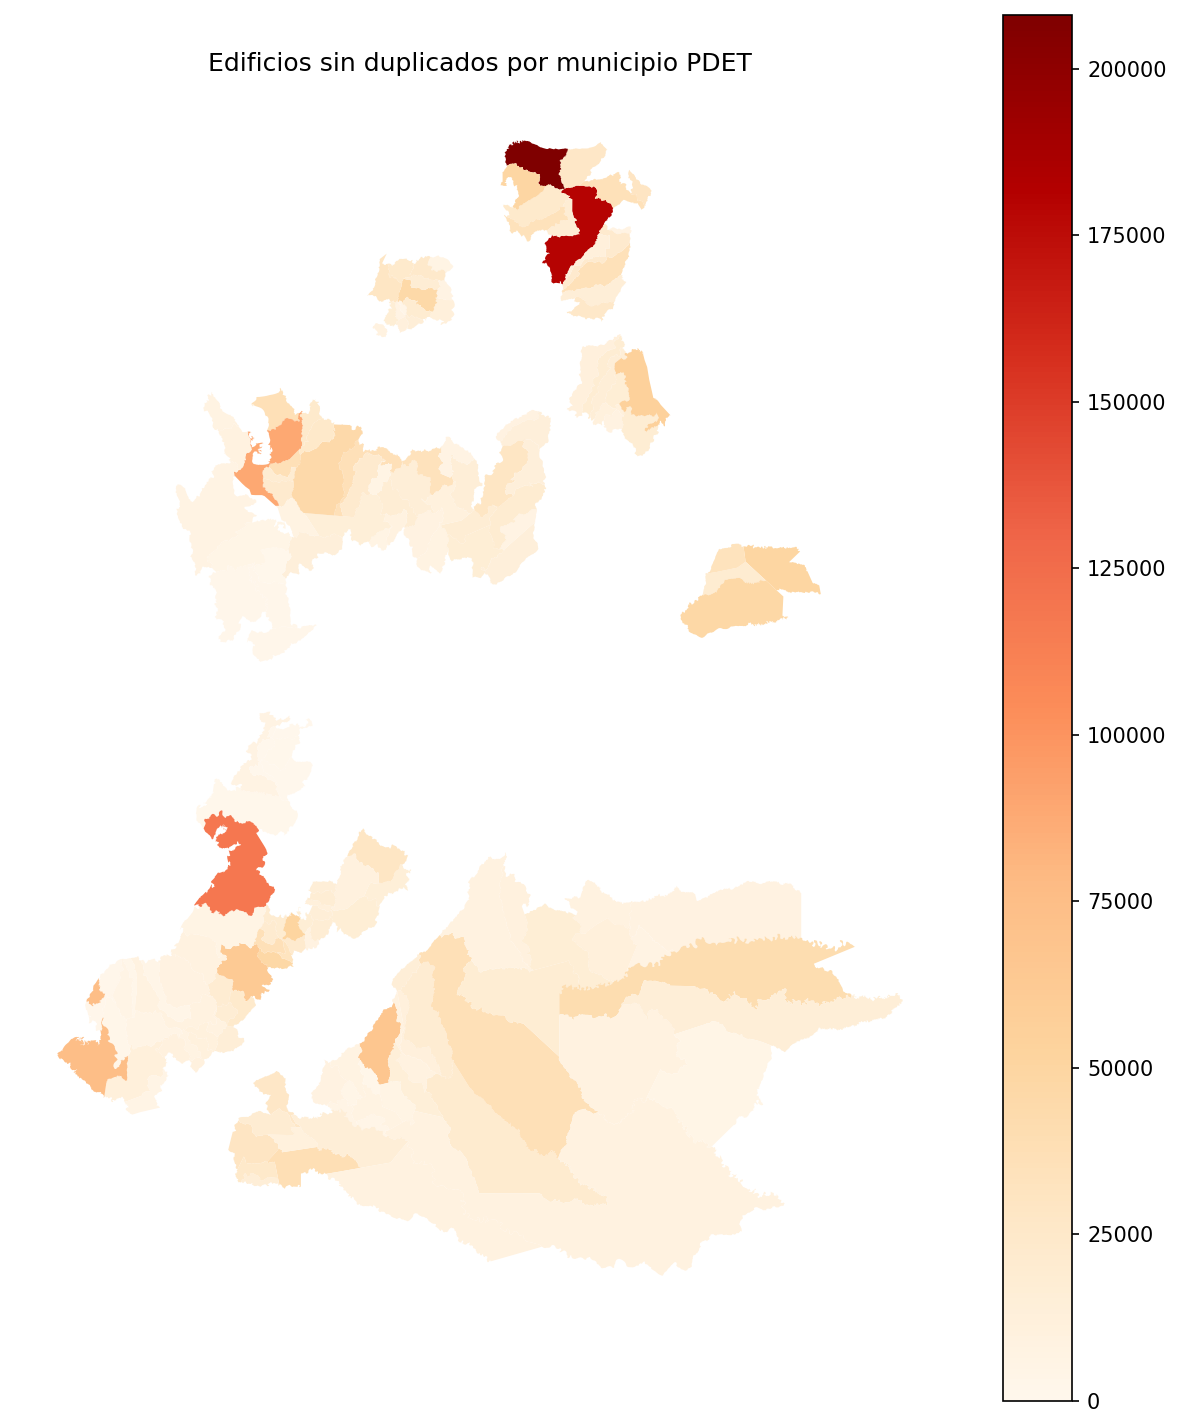
\includegraphics[width=0.82\linewidth]{Imagenes/mapa_rooftop_count.png}
    \caption{Mapa de edificios sin duplicados por municipio PDET. El resultado consolida Google Open Buildings y Microsoft Building Footprints evitando doble conteo por solapamiento espacial.}
    \label{fig:mapa_rooftop_count}
\end{figure}

\begin{figure}[H]
    \centering
    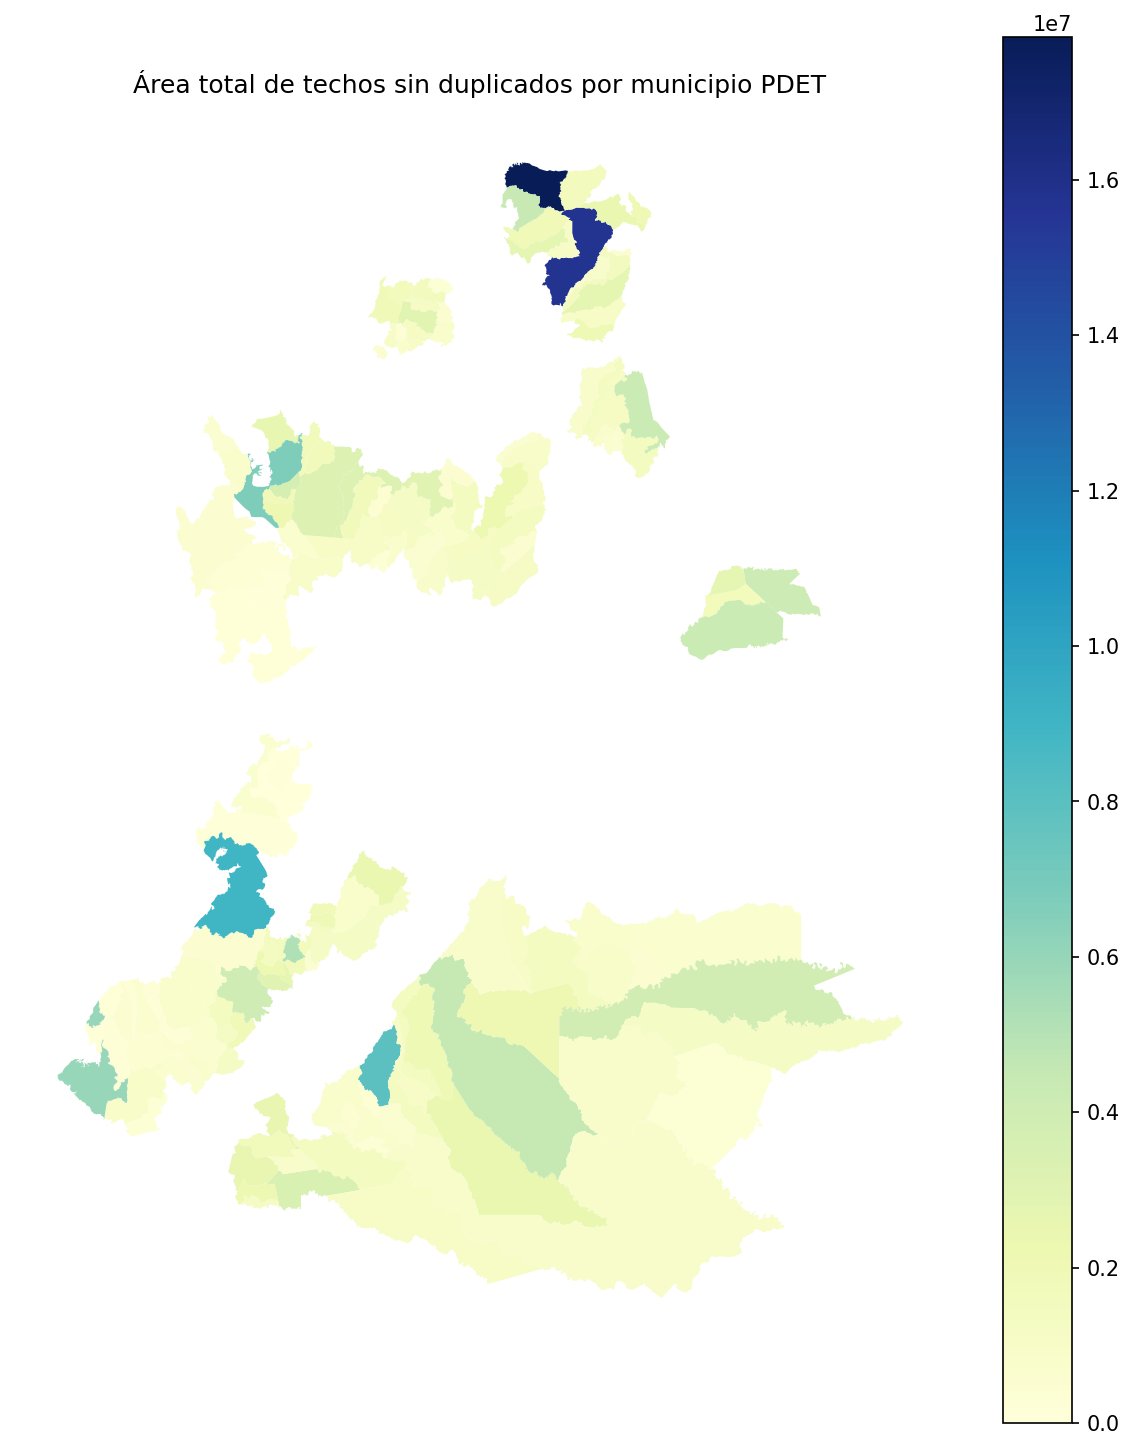
\includegraphics[width=0.82\linewidth]{Imagenes/mapa_rooftop_area.png}
    \caption{Mapa de área total de techos sin duplicados por municipio PDET, calculada en metros cuadrados mediante el sistema de referencia \texttt{EPSG:9377}.}
    \label{fig:mapa_rooftop_area}
\end{figure}

\subsection{Metadatos y reproducibilidad}

Con el objetivo de asegurar trazabilidad y reproducibilidad científica, cada ejecución genera automáticamente un archivo:

\begin{center}
\texttt{run\_metadata.json}
\end{center}

Este archivo almacena:

\begin{itemize}
    \item Fecha y hora UTC de ejecución.
    \item Parámetros utilizados.
    \item Versiones de librerías geoespaciales.
    \item Número de geometrías procesadas.
    \item Metodología aplicada.
\end{itemize}

Un extracto del archivo generado se muestra a continuación:

\begin{lstlisting}[language=Python, caption={Metadatos de ejecución reproducible final}]
{
    "goal": "Estimate count and total rooftop area per PDET municipality.",
    "area_calculation": "Areas calculated using projected CRS EPSG:9377.",
    "deduplication": {
        "threshold": 0.5,
        "priority": "Google is kept as primary source; non-duplicate Microsoft
        buildings are added."
    },
    "global_summary": {
        "google_original_buildings": 2687624,
        "microsoft_original_buildings": 1537635,
        "microsoft_duplicates_with_google": 764492,
        "microsoft_unique_added": 773143,
        "final_buildings_without_duplicates": 3460767,
        "total_rooftop_area_m2": 282191579.71
    }
}
\end{lstlisting}

\subsection{Resultados generales del análisis}

La ejecución del pipeline permitió consolidar información geoespacial 
reproducible sobre el potencial de techos en municipios PDET.

Los principales resultados obtenidos incluyen:

\begin{itemize}
    \item Procesamiento de \textbf{4.225.259} huellas de edificios 
    provenientes de Google Open Buildings y Microsoft Building Footprints.
    \item Identificación de \textbf{764.492} huellas de Microsoft duplicadas 
    con Google mediante solapamiento espacial.
    \item Consolidación de \textbf{3.460.767} edificios finales sin duplicados 
    en los 170 municipios PDET.
    \item Estimación de \textbf{282.191.579,71 m\textsuperscript{2}} de área 
    total de techos sin duplicados (282,19 km\textsuperscript{2}).
    \item Producción automática de capas geoespaciales y reportes reproducibles 
    para análisis posterior.
\end{itemize}

Estos resultados constituyen la base para futuros análisis de potencial 
fotovoltaico y planeación energética territorial dentro del marco PDET.
Estos resultados constituyen la base para futuros análisis de potencial fotovoltaico y planeación energética territorial dentro del marco PDET.

\subsection{Hallazgos territoriales del análisis de rooftops}

El análisis reproducible permitió identificar diferencias significativas en la 
distribución territorial de edificaciones dentro de los municipios PDET. A partir 
de los resultados agregados obtenidos en el archivo 
\texttt{rooftop\_by\_municipio\_deduplicated.csv}, se consolidó el resultado oficial 
de la versión deduplicada, en la cual Google Open Buildings se conserva como fuente 
principal y Microsoft Building Footprints actúa como fuente complementaria. Las 
huellas de Microsoft con solapamiento significativo respecto a Google fueron excluidas 
del conteo final para evitar doble contabilización de techos.

El resultado consolidado comprende \textbf{3.460.767 edificios} distribuidos en los 
170 municipios PDET, con un área total de techos de \textbf{282.191.579,71 m²} 
(282,19 km²), calculada geométricamente mediante proyección al sistema de referencia 
métrico EPSG:9377. Cabe destacar que, dado que Microsoft Building Footprints no 
provee el atributo \texttt{area\_in\_meters} para Colombia —reportando valores de 
\texttt{-1} en los campos \texttt{height} y \texttt{confidence}—, el área de sus 
huellas fue estimada directamente a partir de la geometría poligonal proyectada, 
manteniendo consistencia metodológica con el tratamiento aplicado al dataset de Google.

El Cuadro~\ref{tab:top20_edificios} presenta los 20 municipios con mayor número de 
edificios detectados en el resultado consolidado sin duplicados, mientras que el 
Cuadro~\ref{tab:top20_area} muestra los 20 municipios con mayor área total de techos.

\begin{table}[H]
\centering
\caption{Top 20 municipios PDET por cantidad de edificios --- Resultado consolidado 
sin duplicados (Google + Microsoft)}
\label{tab:top20_edificios}
\small
\begin{tabular}{clrrrr}
\toprule
\textbf{\#} & \textbf{Municipio} & \textbf{Edificios} & \textbf{Área total (m²)} & 
\textbf{Área (ha)} & \textbf{Área (km²)} \\
\midrule
1  & Santa Marta            & 208.108 & 17.841.495,91 & 1.784,15 & 17,84 \\
2  & Valledupar             & 179.817 & 15.701.777,68 & 1.570,18 & 15,70 \\
3  & Buenaventura           & 118.398 &  8.928.950,99 &   892,90 &  8,93 \\
4  & Turbo                  &  89.360 &  6.748.184,75 &   674,82 &  6,75 \\
5  & San Andrés de Tumaco   &  75.652 &  5.965.839,22 &   596,58 &  5,97 \\
6  & Florencia              &  66.892 &  7.941.304,45 &   794,13 &  7,94 \\
7  & El Tambo               &  62.008 &  4.062.485,54 &   406,25 &  4,06 \\
8  & Tibú                   &  54.977 &  4.236.220,06 &   423,62 &  4,24 \\
9  & Santander de Quilichao &  50.580 &  5.220.381,38 &   522,04 &  5,22 \\
10 & Arauquita              &  49.748 &  4.148.534,76 &   414,85 &  4,15 \\
11 & Ciénaga                &  49.248 &  4.443.834,55 &   444,38 &  4,44 \\
12 & Cajibío                &  47.590 &  2.940.102,91 &   294,01 &  2,94 \\
13 & Tame                   &  47.543 &  4.199.296,54 &   419,93 &  4,20 \\
14 & El Carmen de Bolívar   &  45.809 &  2.923.709,67 &   292,37 &  2,92 \\
15 & Tierralta              &  45.262 &  3.209.412,14 &   320,94 &  3,21 \\
16 & San José del Guaviare  &  41.264 &  3.852.209,86 &   385,22 &  3,85 \\
17 & Puerto Asís            &  37.583 &  3.428.869,10 &   342,89 &  3,43 \\
18 & Apartadó               &  36.883 &  3.630.475,29 &   363,05 &  3,63 \\
19 & San Vicente del Caguán &  36.855 &  4.468.540,10 &   446,85 &  4,47 \\
20 & Necoclí                &  36.850 &  2.602.735,74 &   260,27 &  2,60 \\
\bottomrule
\multicolumn{6}{l}{\footnotesize Fuente: elaboración propia a partir de Google Open 
Buildings v3 y Microsoft Building Footprints.} \\
\multicolumn{6}{l}{\footnotesize Áreas calculadas en EPSG:9377. Deduplicación 
espacial con umbral IoU $\geq$ 0,50.} \\
\end{tabular}
\end{table}

\begin{table}[H]
\centering
\caption{Top 20 municipios PDET por área total de techos --- Resultado consolidado 
sin duplicados (Google + Microsoft)}
\label{tab:top20_area}
\small
\begin{tabular}{clrrrr}
\toprule
\textbf{\#} & \textbf{Municipio} & \textbf{Área total (m²)} & \textbf{Área (ha)} & 
\textbf{Área (km²)} & \textbf{Edificios} \\
\midrule
1  & Santa Marta            & 17.841.495,91 & 1.784,15 & 17,84 & 208.108 \\
2  & Valledupar             & 15.701.777,68 & 1.570,18 & 15,70 & 179.817 \\
3  & Buenaventura           &  8.928.950,99 &   892,90 &  8,93 & 118.398 \\
4  & Florencia              &  7.941.304,45 &   794,13 &  7,94 &  66.892 \\
5  & Turbo                  &  6.748.184,75 &   674,82 &  6,75 &  89.360 \\
6  & San Andrés de Tumaco   &  5.965.839,22 &   596,58 &  5,97 &  75.652 \\
7  & Santander de Quilichao &  5.220.381,38 &   522,04 &  5,22 &  50.580 \\
8  & San Vicente del Caguán &  4.468.540,10 &   446,85 &  4,47 &  36.855 \\
9  & Ciénaga                &  4.443.834,55 &   444,38 &  4,44 &  49.248 \\
10 & Tibú                   &  4.236.220,06 &   423,62 &  4,24 &  54.977 \\
11 & Tame                   &  4.199.296,54 &   419,93 &  4,20 &  47.543 \\
12 & Arauquita              &  4.148.534,76 &   414,85 &  4,15 &  49.748 \\
13 & El Tambo               &  4.062.485,54 &   406,25 &  4,06 &  62.008 \\
14 & San José del Guaviare  &  3.852.209,86 &   385,22 &  3,85 &  41.264 \\
15 & Apartadó               &  3.630.475,29 &   363,05 &  3,63 &  36.883 \\
16 & Puerto Asís            &  3.428.869,10 &   342,89 &  3,43 &  37.583 \\
17 & Tierralta              &  3.209.412,14 &   320,94 &  3,21 &  45.262 \\
18 & Montelíbano            &  3.140.424,82 &   314,04 &  3,14 &  36.211 \\
19 & Caucasia               &  2.973.872,32 &   297,39 &  2,97 &  33.540 \\
20 & Cajibío                &  2.940.102,91 &   294,01 &  2,94 &  47.590 \\
\bottomrule
\multicolumn{6}{l}{\footnotesize Fuente: elaboración propia a partir de Google Open 
Buildings v3 y Microsoft Building Footprints.} \\
\multicolumn{6}{l}{\footnotesize Áreas calculadas en EPSG:9377. Deduplicación 
espacial con umbral IoU $\geq$ 0,50.} \\
\end{tabular}
\end{table}

Entre los principales hallazgos obtenidos se destacan:

\begin{itemize}
    \item \textbf{Alta concentración de edificaciones en zonas urbanas consolidadas}: 
    Santa Marta (208.108 edificios) y Valledupar (179.817 edificios) lideran el 
    ranking consolidado, concentrando conjuntamente el 11,2\% del total de 
    edificaciones detectadas en los 170 municipios PDET.

    \item \textbf{Divergencia entre cantidad y área}: Florencia ocupa el puesto 6 
    por número de edificios pero asciende al puesto 4 por área total de techos 
    (7.941.304,45 m²), lo que sugiere una mayor proporción de construcciones de 
    gran superficie, potencialmente industriales o institucionales, con alto 
    potencial fotovoltaico por unidad de edificación.

    \item \textbf{Distribución desigual del área total de techos}: los dos primeros 
    municipios por área (Santa Marta y Valledupar) concentran más de 33,5 km² de 
    superficie de techos, equivalente al 11,9\% del área total estimada para el 
    conjunto PDET.

    \item \textbf{Cobertura territorial heterogénea}: municipios ubicados en 
    regiones selváticas del Pacífico y la Amazonía presentaron menores densidades 
    de detección, coincidiendo con limitaciones de visibilidad satelital y 
    dispersión poblacional características de estas zonas.

    \item \textbf{Mayor cobertura del dataset de Google}: Google Open Buildings 
    detectó aproximadamente 1,75 veces más edificaciones que Microsoft en el 
    conjunto procesado, aportando el 77,7\% del resultado final consolidado.

    \item \textbf{Consistencia espacial}: la tasa de asignación territorial 
    mediante operaciones espaciales \texttt{within} confirmó alta coherencia entre 
    las geometrías de edificios y los límites municipales PDET, con 164 geometrías 
    válidas sobre 164 procesadas (tasa de error: 0\%).
\end{itemize}

El análisis de áreas acumuladas permite estimar que los 170 municipios PDET 
disponen de \textbf{282,19 km²} de superficie de techos potencialmente aprovechable 
para generación fotovoltaica distribuida. Municipios con alta concentración de 
edificaciones y condiciones favorables de radiación solar —como Santa Marta, 
Valledupar y Florencia— se convierten en candidatos estratégicos prioritarios para 
iniciativas de transición energética en el marco PDET.

Adicionalmente, el uso de métricas reproducibles y exportaciones geoespaciales en 
formatos abiertos (GeoJSON, CSV) facilita futuras etapas de modelamiento energético, 
simulación fotovoltaica y priorización territorial por parte de la UPME.



% -------------------- Secciones movidas al final: Comparación, Recomendaciones, Conclusión --------------------
\clearpage
\section{Comparación de Fuentes de Datos de Edificaciones}

Con el fin de seleccionar la fuente más adecuada para la estimación del potencial solar en municipios PDET, se realizó una comparación conceptual y cuantitativa entre los conjuntos de datos Google Open Buildings y Microsoft Building Footprints, orientada al objetivo específico del proyecto: estimar el potencial solar en municipios PDET.

Google Open Buildings se caracteriza por ofrecer una cobertura amplia y uniforme obtenida mediante modelos de inteligencia artificial aplicados sobre imágenes satelitales. Esta fuente presenta alta disponibilidad en regiones en desarrollo y está diseñada para facilitar análisis a gran escala mediante formatos comprimidos optimizados para procesos masivos.

Por otra parte, Microsoft Building Footprints se enfoca en la detección precisa de huellas de edificaciones utilizando imágenes de alta resolución y modelos de visión computacional. En zonas donde sus datos están disponibles, suele entregar geometrías más detalladas y representaciones de forma más precisa de los edificios.

Para el caso específico de Colombia y de los territorios PDET, Google Open Buildings mostró una ventaja en cobertura territorial —en particular en áreas rurales—, lo que lo convierte en una fuente idónea para la identificación inicial de edificaciones a escala nacional. Microsoft Building Footprints, cuando está presente, aporta detecciones complementarias de mayor detalle geométrico que resultan útiles para validación y control de calidad.

La comparación numérica se resume en la siguiente tabla, construida a partir de los resultados consolidados del proyecto:

\begin{table}[H]
\centering
\caption{Comparación numérica entre Google Open Buildings y 
Microsoft Building Footprints}
\begin{tabular}{p{6cm} r r}
\toprule
\tblhdr{Métrica} & \tblhdr{Google} & \tblhdr{Microsoft} \\
\midrule
Edificios cargados & 2.687.624 & 1.537.635 \\
\rowcolor{grisfilas}
Edificios duplicados entre fuentes & -- & 764.492 \\
Edificios únicos aportados al resultado final & 2.687.624 & 773.143 \\
\rowcolor{grisfilas}
Total consolidado sin duplicados & \multicolumn{2}{r}{\textbf{3.460.767}} \\
\bottomrule
\end{tabular}
\end{table}

En términos de cobertura bruta, Google aportó aproximadamente 1.75 veces más edificaciones que Microsoft en el conjunto procesado. Sin embargo, Microsoft añadió más de 770 mil huellas únicas que enriquecen el resultado final y evidencian que ambas fuentes cumplen un rol complementario.

En consecuencia, la estrategia recomendada por este proyecto es:

Para interpretar mejor ese resultado, también conviene observar el peso relativo de cada fuente sobre el total procesado y sobre el resultado final consolidado:

\begin{table}[H]
\centering
\caption{Participación porcentual de cada fuente en el proceso}
\begin{tabular}{p{7cm} r r}
\toprule
\tblhdr{Métrica} & \tblhdr{Google} & \tblhdr{Microsoft} \\
\midrule
Participación sobre el total procesado 
(4.225.259 huellas) & 63,6\% & 36,4\% \\
\rowcolor{grisfilas}
Participación sobre el resultado final sin duplicados 
(3.460.767 edificios) & 77,7\% & 22,3\% \\
\bottomrule
\end{tabular}
\end{table}

\begin{itemize}
    \item Utilizar Google Open Buildings como fuente principal para estimaciones iniciales del potencial solar a escala nacional y para la identificación masiva de techos en municipios PDET.
    \item Emplear Microsoft Building Footprints como fuente complementaria de validación y para enriquecer la muestra en municipios donde sus detecciones estén disponibles.
    \item Mantener una política de deduplicación espacial (ver sección de metodología) en la que, ante solapamientos significativos, se priorice la geometría de Google para conservar continuidad en la base de referencia y se añadan huellas únicas de Microsoft.
\end{itemize}

\section{Recomendaciones para la UPME}

A partir del análisis geoespacial realizado sobre los 170 municipios PDET, 
se presentan las siguientes recomendaciones técnicas a la Unidad de 
Planeación Minero Energética (UPME):

\begin{enumerate}

    \item \textbf{Priorizar Santa Marta, Valledupar y Florencia como municipios 
    piloto para proyectos fotovoltaicos distribuidos.} Estos tres municipios 
    concentran respectivamente 17,84 km², 15,70 km² y 7,94 km² de área total 
    de techos, representando en conjunto el 14,7\% de los 282,19 km² estimados 
    para el total de territorios PDET. Su alta densidad de edificaciones y 
    consolidación urbana los convierten en los candidatos con mayor viabilidad 
    técnica para una fase piloto de generación solar descentralizada.

    \item \textbf{Adoptar Google Open Buildings como fuente base para 
    identificación masiva de techos en territorios PDET.} En el análisis 
    realizado, Google detectó 2.687.624 edificios frente a 1.537.635 de 
    Microsoft, aportando el 77,7\% del resultado final consolidado de 
    3.460.767 edificios. Su cobertura es especialmente superior en municipios 
    rurales y zonas de difícil acceso, donde Microsoft presentó subdetección 
    significativa, como se evidenció en Valledupar (ratio Google/Microsoft 
    de 11,45x) y Tierralta (10,29x).

    \item \textbf{Complementar el análisis con Microsoft Building Footprints 
    para municipios con baja cobertura de Google.} En 36 de los 168 municipios 
    con cobertura en ambas fuentes, Microsoft superó a Google en número de 
    detecciones. Microsoft aportó 773.143 edificios únicos al resultado final, 
    equivalentes al 22,3\% del consolidado. Ignorar esta fuente implicaría 
    subestimar el potencial solar en municipios como Ataco, López y Rioblanco, 
    donde Google presenta menor cobertura.

    \item \textbf{Incorporar datos de radiación solar y demanda energética 
    para una estimación precisa del potencial fotovoltaico.} Los 282,19 km² 
    de área total de techos estimados representan la superficie máxima 
    disponible, pero la superficie técnicamente aprovechable depende de 
    factores como irradiación horizontal global (GHI), orientación e 
    inclinación de techos, y demanda energética local. Se recomienda cruzar 
    los resultados obtenidos con el Atlas de Radiación Solar del IDEAM para 
    obtener estimaciones de generación en kWh por municipio.

    \item \textbf{Mantener y escalar la infraestructura NoSQL geoespacial 
    implementada.} La arquitectura MongoDB con índices \texttt{2dsphere} 
    demostró capacidad para procesar 4.225.259 huellas de edificios 
    distribuidas en 170 municipios, con inserción optimizada por lotes de 
    20.000 documentos e identificación de 764.492 duplicados mediante 
    solapamiento espacial. Esta infraestructura es escalable al conjunto 
    completo de municipios colombianos (1.122 según el MGN 2025) sin 
    cambios arquitectónicos, lo que la convierte en una plataforma 
    sostenible para futuras etapas del análisis energético territorial.

\end{enumerate}


\section{Conclusión}

Este proyecto diseñó e implementó una arquitectura NoSQL geoespacial 
orientada al análisis del potencial solar en techos de edificaciones 
dentro de los territorios priorizados por los Programas de Desarrollo 
con Enfoque Territorial (PDET) en Colombia. A lo largo de cinco etapas 
—diseño del esquema, integración territorial, adquisición de datos, 
carga en MongoDB y análisis reproducible— se construyó un pipeline 
completo, documentado y reproducible que responde directamente al 
objetivo planteado por la UPME.

El resultado central del proyecto es la estimación de \textbf{3.460.767 
edificios} y \textbf{282,19 km² de área total de techos} distribuidos 
en los \textbf{170 municipios PDET}, obtenida mediante la consolidación 
deduplicada de Google Open Buildings (2.687.624 edificios) y Microsoft 
Building Footprints (1.537.635 edificios), con identificación y exclusión 
de 764.492 huellas duplicadas mediante una regla de solapamiento espacial 
con umbral IoU $\geq$ 0,50.

La evaluación comparativa de fuentes evidenció que Google Open Buildings 
constituye la fuente más adecuada para caracterizaciones a escala nacional, 
aportando el 77,7\% del resultado final consolidado y mostrando cobertura 
superior en zonas rurales y de difícil acceso. Microsoft Building Footprints, 
por su parte, cumplió un rol complementario estratégico al agregar 773.143 
edificios únicos no detectados por Google, enriqueciendo el análisis en 
municipios con subdetección de la fuente principal.

Desde el punto de vista metodológico, la decisión de calcular las áreas 
de techos de Microsoft geométricamente —mediante proyección al sistema de 
referencia EPSG:9377— garantizó consistencia en la estimación de superficies 
ante la ausencia del atributo \texttt{area\_in\_meters} en los archivos 
distribuidos para Colombia. Esta decisión, junto con la implementación de 
índices \texttt{2dsphere} y la escritura por lotes de 20.000 documentos, 
permitió procesar eficientemente más de 4,2 millones de huellas dentro de 
una arquitectura MongoDB escalable.

Los municipios de Santa Marta, Valledupar y Florencia se destacan como 
candidatos estratégicos prioritarios, concentrando conjuntamente más de 
41,67 km² de área útil de techos. Estos resultados, exportados en formatos 
abiertos (GeoJSON, CSV) y acompañados de mapas coropléticos reproducibles, 
constituyen una base sólida para que la UPME avance hacia etapas de 
modelamiento fotovoltaico, simulación energética y priorización territorial 
en el marco de la transición energética colombiana.



% -------------------- Fin de secciones movidas --------------------
\end{document}
